\documentclass[11pt]{report}
\usepackage[english, russian]{babel}
\usepackage{xltxtra}
\usepackage{polyglossia}

\usepackage{mathpazo}

\defaultfontfeatures{Ligatures=TeX,Mapping=tex-text}

\setmainfont{STIX2Text-Regular.otf}[
ExternalLocation={/home/vyacheslav/builds/STIXv2.0.2/OTF/},
BoldFont=STIX2Text-Bold.otf,
ItalicFont=STIX2Text-Italic.otf,
BoldItalicFont=STIX2Text-BoldItalic.otf
]
\setmathrm{STIX2Math.otf}[
ExternalLocation={/home/vyacheslav/builds/STIXv2.0.2/OTF/}
]


\usepackage{makeidx}
\usepackage{amssymb, amsthm}
\usepackage{amsmath}
\usepackage{mathtools}
\usepackage{needspace}
\usepackage{enumitem}
\usepackage{cancel}
\usepackage{fdsymbol}
\usepackage{fontawesome}


% разметка страницы и колонтитул
\usepackage[left=2cm,right=2cm,top=1cm,bottom=1.1cm,bindingoffset=0cm]{geometry}
\usepackage{fancybox,fancyhdr}
\fancyhf{}
\fancyhead[R]{\thepage}
\fancyhead[L]{\rightmark}
\fancyfoot{}
\fancyhfoffset{0pt}
\addtolength{\headheight}{13pt}
\pagestyle{fancy}

% Отступы
\setlength{\parindent}{3ex}
\setlength{\parskip}{3pt}

\usepackage{graphicx}
\usepackage{hyperref}

\usepackage{import}
\usepackage{xifthen}
\usepackage{pdfpages}

\newcommand{\incfig}[1]{%
    \def\svgwidth{\columnwidth}
    \import{./figures/}{#1.pdf_tex}
}


\usepackage{xifthen}
\makeatother
\def\@lecture{}%
\newcommand{\lecture}[3]{
    \ifthenelse{\isempty{#3}}{%
        \def\@lecture{Лекция #1}%
    }{%
        \def\@lecture{Лекция #1: #3}%
    }%
    \subsection*{\@lecture}
    \marginpar{\small\textsf{\mbox{#2}}}
}
\makeatletter


\usepackage{xcolor}
\definecolor{Aquamarine}{cmyk}{50, 0, 17, 100}
\definecolor{ForestGreen}{cmyk}{76, 0, 76, 45}
\definecolor{Pink}{cmyk}{0, 100, 0, 0}
\definecolor{Cyan}{cmyk}{56, 0, 0, 100}
\definecolor{Gray}{gray}{0.3}


\usepackage{mdframed}
\mdfsetup{skipabove=3pt,skipbelow=3pt}
\mdfdefinestyle{defstyle}{%
    linecolor=red,
	linewidth=3pt,rightline=false,topline=false,bottomline=false,%
    frametitlerule=false,%
    frametitlebackgroundcolor=red!0,%
    innertopmargin=4pt,innerbottommargin=4pt,innerleftmargin=7pt
    frametitlebelowskip=1pt,
    frametitleaboveskip=3pt,
}
\mdfdefinestyle{thmstyle}{%
    linecolor=cyan!100,
	linewidth=2pt,topline=false,bottomline=false,%
    frametitlerule=false,%
    frametitlebackgroundcolor=cyan!20,%
    innertopmargin=4pt,innerbottommargin=4pt,
    frametitlebelowskip=1pt,
    frametitleaboveskip=3pt,
}
\theoremstyle{definition}
\mdtheorem[style=defstyle]{defn}{Определение}

\newmdtheoremenv[nobreak=true,backgroundcolor=Aquamarine!10,linewidth=0pt,innertopmargin=0pt,innerbottommargin=7pt]{cor}{Следствие}
\newmdtheoremenv[nobreak=true,backgroundcolor=CarnationPink!20,linewidth=0pt,innertopmargin=0pt,innerbottommargin=7pt]{desc}{Описание}
\newmdtheoremenv[nobreak=true,backgroundcolor=Gray!10,linewidth=0pt,innertopmargin=0pt,innerbottommargin=7pt,font={\small}]{ex}{Пример}
\newmdtheoremenv[nobreak=false,backgroundcolor=Cyan!10,linewidth=0pt,innertopmargin=0pt,innerbottommargin=7pt]{thm}{Теорема}
\newmdtheoremenv[nobreak=true,backgroundcolor=Pink!10,linewidth=0pt,innertopmargin=0pt,innerbottommargin=7pt]{lm}{Лемма}

\newtheorem*{st}{Утверждение}
\newtheorem*{prop}{Свойства}

\theoremstyle{plain}
\newtheorem*{name}{Обозначение}

\theoremstyle{remark}
\newtheorem*{rem}{Ремарка}
\newtheorem*{com}{Комментарий}
\newtheorem*{note}{Замечание}
\newtheorem*{prac}{Упражнение}
\newtheorem*{probl}{Задача}


\renewcommand{\proofname}{Доказательство}
\renewenvironment{proof}
{ \hspace{\stretch{1}}\\ \faSquareO\quad \small  }
{ \hspace{\stretch{1}}  \faSquare \normalsize }


\numberwithin{ex}{section}
\numberwithin{thm}{section}
\numberwithin{equation}{section}



\newcommand{\K}{\mathcal{K}}
\newcommand{\Z}{\mathbb{Z}}
\newcommand{\N}{\mathbb{N}}
\newcommand{\Real}{\mathbb{R}}
\newcommand{\Q}{\mathbb{Q}}
\newcommand{\Cm}{\mathbb{C}}
\newcommand{\Pm}{\mathbb{P}}
\newcommand{\ord}{\operatorname{ord}}
\newcommand{\lcm}{\operatorname{lcm}}
\newcommand{\sign}{\operatorname{sign}}
\newcommand{\E}{\mathbb{E}}

\renewcommand{\o}{o}
\renewcommand{\O}{\mathcal{O}}
\renewcommand{\le}{\leqslant}
\renewcommand{\ge}{\geqslant}

\def\mybf#1{\textbf{#1}}
\def\selectedFont#1{\textbf{#1}}
\def\ComplexityFont#1{\textmd{\textbf{\textsf{#1}}}}
\def\LanguageFont#1{{\textbf{\texttt{#1}}}}


\newcommand{\Cclass}{\mathcal{C}}
\newcommand{\Dclass}{\mathcal{D}}


\renewcommand{\P}{\ComplexityFont{P}}
\newcommand{\DTIME}{\ComplexityFont{DTime}}
\newcommand{\DTime}{\ComplexityFont{DTime}}
\newcommand{\DSpace}{\ComplexityFont{DSpace}}
\newcommand{\PSPACE}{\ComplexityFont{PSPACE}}
\newcommand{\NTIME}{\ComplexityFont{NTime}}
\newcommand{\NSpace}{\ComplexityFont{NSpace}}
\newcommand{\coNSpace}{\ComplexityFont{coNSpace}}
\newcommand{\NPSPACE}{\ComplexityFont{NPSPACE}}
\newcommand{\poly}{\ComplexityFont{poly}}
\newcommand{\RP}{\ComplexityFont{RP}}
\newcommand{\coRP}{\ComplexityFont{co-RP}}
\newcommand{\ZPP}{\ComplexityFont{ZPP}}
\newcommand{\BPP}{\ComplexityFont{BPP}}
\newcommand{\BQP}{\ComplexityFont{BQP}}
\newcommand{\coBPP}{\ComplexityFont{co-BPP}}
\newcommand{\NP}{\ComplexityFont{NP}}
\newcommand{\NL}{\ComplexityFont{NL}}
\newcommand{\coNL}{\ComplexityFont{co-NL}}
\renewcommand{\L}{\ComplexityFont{L}}
\newcommand{\NPcomp}{\ComplexityFont{NP-complete}}
\newcommand{\tP}{\widetilde{\P}}
\newcommand{\tNP}{\widetilde{\NP}}
\newcommand{\tBH}{\widetilde{\BH}}
\newcommand{\Class}{{\ComplexityFont{C}}}
\newcommand{\coC}{\ComplexityFont{co-}\mathcal{C}}
\newcommand{\coNP}{\ComplexityFont{co-NP}}
\newcommand{\PH}{\ComplexityFont{PH}}
\newcommand{\EXP}{\ComplexityFont{EXP}}
\newcommand{\Size}{\ComplexityFont{Size}}
\newcommand{\Ppoly}{\ComplexityFont{P}/\ComplexityFont{poly}}
\newcommand{\NC}{\ComplexityFont{NC}}


\newcommand{\FACTOR}{\LanguageFont{FACTOR}}
\newcommand{\kQBF}{{\LanguageFont{QBF{\tiny k}}}}
\newcommand{\QBFk}{{\LanguageFont{QBF{\tiny k}}}}
\newcommand{\QBF}{{\LanguageFont{QBF}}}
\newcommand{\STCON}{\LanguageFont{STCON}}
\newcommand{\USTCON}{\LanguageFont{USTCON}}
\newcommand{\CircuitSat}{{\LanguageFont{CIRCUIT\_SAT}}}
\newcommand{\tCircuitSat}{\widetilde{{\LanguageFont{CIRCUIT\_SAT}}}}
\newcommand{\SAT}{\LanguageFont{SAT}}
\newcommand{\tSAT}{\widetilde{{\LanguageFont{SAT}}}}
\newcommand{\UNSAT}{{\LanguageFont{UNSAT}}}
\newcommand{\tThreeSAT}{\widetilde{{\LanguageFont{3\text{-}SAT}}}}
\newcommand{\ThreeSAT}{{\LanguageFont{3\text{-}SAT}}}
\newcommand{\BH}{\LanguageFont{BH}}
\newcommand{\CircuitEval}{{\LanguageFont{CIRCUIT\_EVAL}}}


\newcommand{\const}{\textmd{const}}
\newcommand{\logspace}{\textmd{logspace}}
\newcommand{\PATH}{\textmd{PATH}}


\newcommand{\readonly}{\textsf{read-only}}
\newcommand{\writeonly}{\textsf{write-only}}


\usepackage{ upgreek }
\newcommand{\PI}{\Uppi}
\newcommand{\SIGMA}{\Upsigma}
\newcommand{\DELTA}{\Updelta}

\input{pythonhighlight.tex}

\title{Конспект по теории вычислимости\\IV семестр, 2021 год\\
    Современное программирование, факультет математики и компьютерных наук, СПбГУ\\
(лекции Пузыниной Светланы Александровны)}
\author{Тамарин Вячеслав}

\makeindex
\begin{document}
\maketitle
\tableofcontents
\hspace{1em}
\begin{center}
	Исходный код на \url{https://github.com/tamarinvs19/theory_university}
\end{center}
\begin{center}
	\textbf{
    Некоторые доказательства были опущены на лекции, но написаны мной. Они выделены оранжевыми символами:
}
	\begin{proof*}
		Исправляйте, дополняйте. Чем меньше недоказанных утверждений, тем лучше!
	\end{proof*}
\end{center}

\printindex
\chapter{Вычислимость. Система вычислимости по Клини} 
\section{Рекурсивные функции}

\lecture{1}{11 feb}{\dag}
\begin{defn}[]\index{$ k$-местная частичная функция}
	Пусть функция $ f\colon \N^{k} \to  \N, ~ k \in \N$, где $ \N = \{0, 1, 2, \ldots \}$\footnote{Мы здесь считаем ноль натуральным числом}. Такая функция называется \selectedFont{$ k $-местной частичной функцией}. Если $ k = 0$, то $ f = \const$.
\end{defn}

\subsection{Простейшие функции} \index{простейшие функции}
\selectedFont{Простейшими} будем называть следующие функции:
\begin{itemize}
	\item Нуль местный нуль --- функция без аргументов, возвращающая $ 0$;
	\item Одноместный нуль --- $ 0(x) = 0$;
	\item Функция следования --- $ s(x) = x + 1$;
	\item Функция выбора (проекция) ---  $ I_{n}^{m}(x_1, \ldots x_{n}) = x_m$
\end{itemize}


\subsection{Операторы}
Определим три оператора:
\begin{defn}
\begin{itemize}
    \item \index{оператор суперпозиции}
	Функция $ f$ \selectedFont{получается оператором суперпозиции} из функций $ h$ и $ g_i$, где
	\[
		h(y_1, \ldots , y_m), ~ g_i(x_1, \ldots , x_n); ~ 1 \le i \le m
	,\] 
	если 
	\[
		f = h(g_1(x_1, \ldots, x_{n}), \ldots g_m(x_1, \ldots , x_{n}))
	.\] 
	Оператор обозначается $\S$.
\item \index{оператор примитивной рекурсии}
	Функция $ f^{(n+1)} $\footnote{Здесь и далее $ f^{(n)}$ обозначается функция, принимающая $ n$ аргументов, то есть $ n$-местная}
	\selectedFont{получается оператором примитивной рекурсией} из $ g^{(n)}$  и $ h^{(n+2)}$, если 
	\[
	\begin{cases}
		f(x_1, \ldots x_{n}, 0) = g(x_1, \ldots x_{n}) \\
		f(x_1, \ldots x_{n}, y+1) = h(x_1, \ldots x_{n}, y, f(x_1, \ldots x_{n}, y))
	\end{cases}
	\] 
	Оператор обозначается $ \R$.
\item \index{оператор минимизации}
	Функция $ f$ задается \selectedFont{оператором минимизации} ($ \M$), если она получается из функции  $ g$:
	\[
	\begin{aligned}
		f(x_1, \ldots x_{n}) & = \mu y \bigl[ g(x_1, \ldots x_{n}, y) = 0 \bigr] = \\
							 &= 
							 \begin{cases}
								 y & g(x_1, \ldots x_{n}, y) = 0 \wedge g(x_1, \ldots x_{n}, i)\footnote{подразумевается, что функция определена в этих точках} \ne 0 ~ \forall i < y \\
								 \uparrow\footnote{не определена} & else
							 \end{cases}
	\end{aligned}
	\]
\end{itemize}
\end{defn}

\begin{ex}
    \[
    x - y = \begin{cases}
		x - y, & x \ge  y \\
		\uparrow, & x < y
    \end{cases}
    \] 
	Можно задать, используя оператор минимизации:
	\[
		x - y = \mu z [\lvert (y+z) - x \rvert = 0]
	.\] 
\end{ex}



\subsection{Функции}
\begin{defn}[Примитивно рекурсивная функция]\index{примитивно рекурсивная функция}
	Функция $ f$ называется \selectedFont{примитивно рекурсивной} (\prf),
	если 
	существует последовательность таких функций  $ f_1, \ldots f_k$, что
	все $ f_i$ либо простейшие, либо получены из предыдущих $ f_1, \ldots f_{i-1}$ с помощью одного из операторов $\S$ и $\R$ и $ f = f_k$.
\end{defn}


\begin{ex}\label{ex:1}
	Докажем, что $ f(x, y) = x + y$ --- \prf. По  $ \R$ можем получить $ f$ так:
	\[
	\begin{cases}
		f(x, 0) &= x = I^{1}_{1} (x) =g \\
		f(x, y+1) &= (x + y) + 1 = s(f(x, y)) = s(I^{3}_{3} (x, y, f(x, y)) = h 
	\end{cases}
	\] 
	Теперь построим последовательность функций $ f_i$, где последним элементом будет $ f$, полученный с помощью $ \R$: 
	\[
		I^{1}_{1} , ~s, ~I^{3}_{3} , ~ h = \S(s, I^{3}_{3}) ,~ f
	.\] 
\end{ex}


\begin{defn}[Частично рекурсивная функция]\index{частично рекурсивная функция}
	Функция $ f$ называется \selectedFont{частично рекурсивной функцией} (\crf), если существует последовательность функций $ f_1, \ldots f_k$, таких что $ f_i$ либо простейшая, либо получается из предыдущих с помощью одного из операторов  $ \S, \R, \M$.
\end{defn}

\begin{note}
    Частично рекурсивная функция может быть не везде определена. Примитивно рекурсивная определена везде.
\end{note}
\begin{note}
    Существуют частично рекурсивные функции, которые всюду определены, но при этом не являются \prf.
\end{note}

\begin{defn}\index{общерекурсивная функция}
	\selectedFont{Общерекурсивная функция} --- всюду определенная частично рекурсивная.
\end{defn}


\begin{ex}
	$ \mu y [x + y + 1 = 0]$ --- нигде не определена, но получается из последовательности других функций с помощью операторов.
\end{ex}



\begin{lm}\label{lm:rec}
    Следующие функции являются \prf:
	\begin{enumerate}
	\item $ \const ^{(n)}$ 
	\item $ x + y$ 
	\item $ x\cdot y$ 
	\item $ x ^{y}$, где $ 0^{0}$ можем определить, как хотим
	\item $ \sg(x) = \begin{cases}
			0 & x= 0 \\
			1 & x\ne 0
		\end{cases}$
	\item $ \bsg(x) = \begin{cases}
			1 & x= 0 \\
			0 & x\ne 0
		\end{cases}$
	\item $ x \dotminus 1 = \begin{cases}
			u & x = 0 \\
			x - 1 & x > 0
		\end{cases}$ 
	\item $ x \dotminus y = \begin{cases}
			0 & x < y \\
			x - y & else
		\end{cases}$ 
	\item $ \lvert x - y \rvert $
	\end{enumerate}
\end{lm}
\begin{proof*}
	\begin{enumerate}
		\item Сначала можем получить нужное число последовательной суперпозицией функции следования (получили константу от одной переменной), затем проецируем $ I^{n + 1}_{1}$, чтобы получить $ n$ переменных (первая - наша константа).
		\item Доказали выше \hyperref[ex:1]{в примере \ref{ex:1}}.
		\item $ f(x, y) = xy$ определим так:
			\[
			\begin{cases}
				f(x, 0) &= 0\\
				f(x, y+1) &= f(x, y) + x
			\end{cases}
			\] 
			а складывать мы умеем.
		\item $ f(x, y) = x^{y}$ :
			\[
			\begin{cases}
				f(x, 0) &= 1 = s(0) \\
				f(x, y+1) &= f(x, y) * y
			\end{cases}
			\] 
			Умножать тоже можно по третьему пункту.
		\item  $ \sg(x) = \begin{cases}
				0&x=0 \\
				1& x\ne 0
		\end{cases}$
		\[
		\begin{cases}
			\sg(0) &= 0 \\
			\sg(x+1) &= 1 = s(0)
		\end{cases}
		\] 
	\item Аналогично
	\item $ f(x) = x \dotminus 1$ 
		\[
		\begin{cases}
			f(0) &=0 \\
			f(x+1) &= x = I^{1}_{1} (x)
		\end{cases}
		\] 
	\item $ f(x, y) = x \dotminus y$
		\[
		\begin{cases}
			f(x, 0) &= x = I^{1}_{1}(x)  \\
			f(x, y+1) &= f(x, y) \dotminus 1
		\end{cases}
		\] 
	\item $ f(x, y) = \lvert x - y \rvert  = (x \dotminus y) + (y \dotminus x)$
    \end{enumerate}
\end{proof*}
\begin{note}
    Обычное вычитание не является \prf, так как не везде определено на $ \N$.
\end{note}



\subsection{Оператор ограниченной минимизации}
\begin{defn}[Оператор ограниченной минимизации]\index{оператор ограниченной минимизации}
	Функция $ f^{(n)}$ задается \selectedFont{оператором ограниченной минимизации} из функций $ g^{(n+1)}$ и $ h^{(n)}$, если
	 \[
		\mu y \le h(\overline{x}) \bigl[ g(\overline{x}, y) = 0\bigr]\footnote{Здесь и далее $ \overline{x} = x_1, \ldots x_{n}$.} \\
	 .\]
	 Это означает, что
	 \[
		 f(\overline{x}) = 
		 \begin{cases}
			 y & g(\overline{x}, y) = 0 \wedge y \le h(\overline{x}) \wedge g(\overline{x}, i) \ne 0\footnote{Аналогично, подразумевается, что функция определена в этих точках} ~ \forall i < y \\
			 h(\overline{x})+1 & else
		 \end{cases}
	 \] 
\end{defn}


\begin{st}
    Пусть $ g^{(n+1)}, h^{(n)}$ --- примитивно рекурсивные функции, и $ f^{(n)}$ получается из $ g$ и $ h$ с помощью ограниченной минимизации, то $ f$ тоже \prf.
\end{st}
\begin{proof*}
	Заметим, что $ f$ можно получить следующим образом:
	\[
		f(\overline{x}) = \sum_{y=0}^{h(x)}	\prod_{i=0}^{y}\sg(g(\overline{x}, i))
	.\] 
	Внутреннее произведение равно единице только тогда, когда все $ g(\overline{x}, i) \ne 0$. 
	Если для некоторого $ y$ обнуляется $ g(\overline{x}, y)$, то все произведения, начиная с $ y+1$, будут равны нулю, поэтому просуммируем только  $ y$ единиц. 
	Если же такого $ y$ нет, получим сумму из $ h(\overline{x}) + 1$ единицы. Именно это и нужно.

	Проверим, что можно получить $$ a(\overline{x}, y) = \sum_{i=0}^{y} g(\overline{x}, i), \quad m(\overline{x}, y) = \prod{i=0}^{y} g(\overline{x}, i)$$ с помощью примитивной рекурсии:
	\[
	\begin{aligned}
		&\begin{cases}
			a(\overline{x}, 0) &= g(\overline{x}, 0) \\
			a(\overline{x}, y+1) &= a(\overline{x}, y) + g(\overline{x}, y+1)
		\end{cases}
		&\begin{cases}
			m(\overline{x}, 0) &= g(\overline{x}, 0) \\
			m(\overline{x}, y+1) &= m(\overline{x}, y) \cdot g(\overline{x}, y+1)
		\end{cases}
	\end{aligned}
	\]
\end{proof*}


\begin{note}
	$ {\color{red}0(x)}$ можно исключить из определения простейших функций, так как ее можно получить с помощью оператора $ \R$ для нульмерного $ {\color{green}0}$ и $ I^{2}_{2} (x, y)$ :
	\[
		{\color{red}0(y)} = 
		\begin{cases}
			{\color{red}0(0)} &= {\color{green}0} \\
			{\color{red}0(y+1)} &=I^{2}_{2} (y, {\color{green}0})
		\end{cases}
	\] 
\end{note}


\subsection{Предикаты}
\begin{defn}\index{предикаты}
	Предикат --- условие задающее подмножество: $ R \subset \N^{k}$.
	
	\noindent
	Предикат называется \selectedFont{примитивно рекурсивным (общерекурсивным)}, его характеристическая функция примитивно рекурсивная (общерекурсивная).
\[
	\chi_{R}(\overline{x})= 
	\begin{cases}
		1, &\overline{x} \in  R \\
		0, &\overline{x} \notin R
	\end{cases}
\] 
\end{defn}


\begin{st}
	~\begin{itemize}
		\item Если  $ R, Q$ --- примитивно рекурсивные (общерекурсивные) предикаты, то предикаты $ P \vee Q$, $P \wedge Q$, $P \to Q$, $\neg P$ тоже примитивно рекурсивные (общерекурсивные).
		\item Предикаты $ = , ~\le , ~\ge , ~<, ~>$ тоже примитивно и общерекурсивны.
    \end{itemize}
\end{st}
\begin{proof*}
	~\begin{itemize}
		\item Проверим, что характеристические функции примитивно / общерекурсивны: 
			\[
			\begin{aligned}
				\chi_{P \wedge  Q}(\overline{x}) & = \chi_{P}(\overline{x}) \cdot \chi_{Q}(\overline{x}) \\
				\chi_{P \vee Q}(\overline{x}) & = \sg(\chi_{P}(\overline{x}) + \chi_{Q}(\overline{x})) \\
				\chi_{P \to Q}(\overline{x}) &= \bsg(\chi_{P}(\overline{x}) + \bsg(\chi_{Q}(\overline{x}))) \\
				\chi_{\neg P} (\overline{x}) & = \bsg(\chi_{P}(\overline{x}))
			\end{aligned}
			\]
		\item Аналогично выразим, через простейшие:  
			\[
			\begin{aligned}
				\chi_{x=y} (x) &= \bsg(\lvert x - y \rvert ) = \begin{cases}
					1, &x=y \\
					0, &x\ne y
				\end{cases} \\
					\chi_{x< y}(x) &= \sg(x \dotminus y)
			\end{aligned}
			\]
			Остальные можем выразить также или через уже проверенные $ <$ и $ \neg$.
    \end{itemize}
\end{proof*}


\begin{lm}
    Следующие функции являются примитивно рекурсивными:
	\begin{enumerate}
		\item $ \left\lfloor \frac{x}{y} \right\rfloor$, считаем, что $ \left\lfloor \frac{x}{0} \right\rfloor = x$
		\item $\Div(x, y) = 
\begin{cases}
	1, & y \mid x \\
	0, & else
\end{cases}$
\item $ \Prime(x) = \begin{cases}
		1, & x \in \Pm\\
		0, & else
\end{cases}$
\item  $ f(x) = p_{x}$, где $ p_{x} $ --- $ x$-тое простое число, $ p_0 \coloneqq  2$
\item  $ \expp(i, x) $ --- степень простого числа $ p_i$ разложении $ x$, $ \expp(i, 0) \coloneqq 0$
	\end{enumerate}
\end{lm}
\begin{proof*}
    \begin{enumerate}
		\item $ f(x, y) = \left\lfloor \frac{x}{y} \right\rfloor $. Найдем минимальное $ k$, что $ f'(x, y, k) = yk > x$. Чтобы получить  $$ f(x, y) = \min(k \mid f'(x, y, k)) - 1,$$ используем оператор минимизации:
			 \[
				 f(x, y) = \mu k [ \neg f'(x, y, k) = 0] - 1
			.\] 
		\item $ \Div(x, y) = \left\lfloor \frac{x}{y} \right\rfloor \cdot y = x$
		\item Определим  $ \Div'(x, y) = (y \le  1) \vee (\neg\Div(x, y))$, эта функция проверяет, что число $ y$ не является нетривиальным делителем $ x$.

			Теперь, используя ограниченную минимизацию, выразим  $ \Prime(x)$ :
			\[
				\Prime(x) = \Bigl(\mu y \le h(x) [\Div'(x, y) = 0]\Bigr) = x, \text{ где } h(x) = x - 1 
				.\]
				То есть мы посмотрели на все меньшие числа, если среди них найдется нетривиальный делитель, то число не простое.
			\item Пусть $ f'(x) = \text{ количество простых } \le x $. 
				\[
					\begin{cases}
						f'(0) &= 0 \\
						f'(x+1) &= \Prime(x+1) + f(x)
					\end{cases}
				\] 
				Теперь можно вычислить $ f(x)$: для этого определим функцию $ g(x, y) = (f'(y) = x)$,
				 \[
					 f(x) = \mu y [ \neg f'(x, y)  = 0] 
				.\] 
			\item Чтобы найти степень вхождения простого числа $ p_i$ в $ x$, сначала находим это простое число по номеру, затем находим минимальное $ k$, что $ x$ не делится на $ p_i^{k}$ и вычитаем единицу.
    \end{enumerate} 
\end{proof*}


\subsection{Теоремы про рекурсии}
\begin{thm}[Канторовская нумерация]
    Пусть $ \pi\colon \N \times \N \to  \N$ :
	\[
		\pi(x, y) = \frac{1}{2}(x+y) (x+y+1)+y
	.\] 
	\begin{itemize}
	\item
	Тогда для любого $ z$ существует единственное представление $ z = \pi(x, y)$.
\item Причем функции $ x(z), y(z)$ примитивно рекурсивные.
	\end{itemize}
\end{thm}
\begin{proof*}
	\begin{itemize}
		\item
	Запишем $ \pi(x, y) = {{x+y+1}\choose{2}} + y$. Заметим, что для $ n > m$ верно  
	$$ {n \choose 2} - {m \choose 2} \ge {n \choose 2} - {n-1 \choose 2} = n-1.$$
	Предположим, что $ x + y >  x' + y'$ и  $ \pi(x, y) = \pi(x',y')$. Тогда
	 \[
		 y' - y = {x+y+1 \choose 2} - {x'+y'+1 \choose 2} \ge x + y > x' + y'
	.\] 
	Но $ y \ge 0, ~ x' \ge 0$,  поэтому $ y' - y \le  y$, а $ x'+y' \ge y'$, а тогда $ y' - y \le x' + y'$, что противоречит полученному выше неравенству.

	Если $ x + y = x' + y'$, то $ 0 = \pi(x, y) - \pi(x', y') = y - y'$. Тогда $ y=y'=0$, поэтому  $ x = x'$. 

	Доказали, что из равенства  $ \pi(x, y) = \pi(x', y')$ следует равенство $ (x, y)= (x', y')$.
\item  Можно по-честному все посчитать и выразить $ x(z), ~y(z)$.
	Пусть 
	\[
	\begin{aligned}
		w &= x+y \\
		t &= \frac{1}{2}w(w+1) = \frac{w^2+w}{2} \\
		z &= t +y
	\end{aligned}
	\]
	Решим квадратное уравнение, чтобы выразить $ w$ через $ t$\footnote{отрицательный корень можем сразу отбросить}:
	\[
		w = \frac{-1 + \sqrt{ 8t + 1}}{2}
	.\] 
	Запишем неравенство:
	\[
		t \le z = t + y < t + (w +1) = \frac{(w+1)^2+(w+1)}{2}
	.\] 
	Аналогично выразим $ w+1$ через $ z$: имеем $ z < \frac{(w+1)^2+(w+1)}{2}$, решаем неравенство, а далее вспоминаем, что все числа положительные и можно забыть про отрицательные корни.
	Отсюда
	\[
		w \le \frac{-1  + \sqrt{ 8z +1} }{2} < w+1
	.\] 
	Тогда 
	\[
	\begin{aligned}
		w &= \left\lfloor \frac{-1 + \sqrt{ 8z+1} }{2} \right\rfloor \\
		t &= \frac{w^2+w}{2} \\
		y &= z - t \\
		x &= w - y
	\end{aligned}
	\]
	Таким образом, мы выразили через $ z$ обе координаты. Единственный момент --- нужно извлекать корень, в натуральную степень возводить мы умеем, поэтому можем с помощью ограниченной минимизации перебрать все меньшие числа, возвести их в квадрат и сравнить с нашим числом.
	\end{itemize}
\end{proof*}


\begin{thm}[Возвратная рекурсия]\index{рекурсия возвратная}
    Зафиксируем $ s$. Пусть 
	\[
	\begin{cases}
		f(\overline{x}, 0) &= g(\overline{x}) \\
		f(\overline{x}, y+1) &= h(\overline{x}, y, f(\overline{x}, t_1(y)), \ldots f(\overline{x}, t_{s}(y)))
	\end{cases}
	\] 
	где $ \forall 1 \le i \le s ~t_i(y) \le y$, $ g^{(n)}, h^{(n+1+s)}, t_i^{(1)}$.

	\noindent
	Тогда, если $ g, h, t_i$ --- примитивно / общерекурсивные, то и $ f$ тоже.
\end{thm}
Основная идея этой теоремы --- можем использовать все ранее вычисленные значения функции, а не только предыдущее.
\begin{proof*}
	Построим с помощью примитивной рекурсии функцию $ m(\overline{x}, y)$, которая возвращает закодированную последовательность $ f(\overline{x}, i), ~ 0 \le i \le y$.

	Кодировать будем так: каждому $ f(\overline{x}, i)$ будет соответствовать $ p_i$ ($ i$-ое простое число) в степени $ 1 + f(\overline{x}, i)$. 

	Если мы построим эту функцию, то $ f(\overline{x}, y)$ --- уменьшенная на $ 1$ степень $ y$-ого простого, обозначим функцию, которая это делает:
	\[
		f(\overline{x}, y) = \ith(y, m(\overline{x}, y))
	.\] 
	Вернемся к построению $ m$:
	\[
	\begin{cases}
		m(\overline{x}, 0) &= 2^{1+g(\overline{x})} \\
		m(\overline{x}, y+1) &= m(\overline{x}, y) \cdot p_{y+1}^{1+h\left( 
			\overline{x}, y, \ith(t_1(y), m(\overline{x}, y)), \ldots \ith(t_{k}(y), m(\overline{x}, y))
	\right)
}
	\end{cases}
	\] 
\end{proof*}


\begin{thm}[Совместная рекурсия]\index{рекурсия совместная}
	Пусть $ f_i^{(n+1)}, ~ 1 \le i \le k$,
	\[
	\begin{cases}
		f_i(\overline{x}, 0) &= g_i(\overline{x}) \\
		f_i(\overline{x}, y+1) &= h_i (\overline{x}, y, f_1(\overline{x}, y), \ldots f_{k}(\overline{x}, y))
	\end{cases}
	\] 
	Если $ g_i^{(n)}, h_i^{(k+2)}, ~1 \le i \le k$ --- примитивно / общерекурсивные, то $ f_i$ тоже.
\end{thm}
Основная идея этой теоремы --- можем использовать $ y$-е значение каждой из $ k$ функций.
\begin{proof*}
	Заметим, что канторовскую функцию можно, последовательно применив несколько раз, расширить до $ k$-местной. Обозначим полученную функцию за $ c$, а обратные за $ c_1, \ldots c_{k}$.

	Давайте просто объединим все $ f_i$ в одну функцию 
	\[
		m (\overline{x}, y) = c\left(f_1(\overline{x}, y), \ldots f_k(\overline{x}, y)\right)
	.\]
	Теперь каждую $ f_i$  можно вычислить
	\[
		f_i(\overline{x}, y) = c_i(m (\overline{x}, y))
	.\] 
	Чтобы получить $ m$ достаточно использовать примитивную рекурсию:
	\[
	\begin{cases}
		m(\overline{x}, 0) &= c\left(g_1(\overline{x}), \ldots g_k(\overline{x})\right) \\
		m(\overline{x}, y+1) &= c ( \\
							 &\quad\begin{aligned}
				&h_1\left( \overline{x}, y, c_1(m(\overline{x}, y)), \ldots c_k(m(\overline{x}, y)) \right), \\
				&\quad\vdots \\
				&h_k\left( \overline{x}, y, c_1(m(\overline{x}, y)), \ldots c_k(m(\overline{x}, y)) \right)
			\end{aligned} \\
							 &) 
	\end{cases}
	\] 
\end{proof*}


\begin{thm}[Кусочное задание функции]\index{кусочное задание функции}
	Пусть $ R_0, \ldots R_k $ --- отношения\footnote{Набор предикатов}, такие что $ \bigsqcup\limits_{i=0}^{k} R_i = \N^{m}$
	\footnote{То есть для $ i \ne  j$ верно $ R_{i} \cap R_j = \varnothing$.}.
	Для $ \lvert \overline{x} \rvert = n$ кусочно зададим функцию $ f^{(n)}$:
\[
	f(\overline{x}) = \begin{cases}
		f_0(\overline{x}), & \text{если }R_0(\overline{x}) \\
		f_1(\overline{x}), &  \text{если }R_1(\overline{x}) \\
		\quad\vdots & \quad\vdots \\
		f_k(\overline{x}), &  \text{если }R_k(\overline{x}) \\
	\end{cases}
\] 
Если $ f_i^{(n)}, R_i$ --- примитивно / общерекурсивны, то и $ f$ тоже.
\end{thm}
\begin{proof*}
	Рассмотрим характеристические функции $ \chi_{R_{i}} $ для $ R_i$.
	Тогда 
	\[
		f(\overline{x}) = \sum_{i=0}^{k} f_i(\overline{x}) \cdot \chi_{R_{i}}(\overline{x})
	.\] 
	А это просто сумма произведений, которые мы можем вычислять.
\end{proof*}


\section{Равносильность МТ и \crf} \index{равносильность МТ и \crf}
\begin{thm}
	Функция вычисляется машиной Тьюринга тогда и только тогда, когда она частично рекурсивная (то есть вычислима по Клини).
\end{thm}
\begin{proof}
    \begin{description}
		\item[\boxed{ 2 \Longrightarrow 1}]
			Если $ f(x_1, \ldots x_n) = y$, то считаем, что МТ получаем $ 1^{x_1}01^{x_2}0\ldots 01^{x_n}$ и должна выдать $ 1^{y}$; если  $ f$ не определена, МТ должна зацикливаться и наоборот.
			\begin{itemize}
				\item Для простых функций можем построить МТ напрямую:
					\begin{itemize}
						\item Если мы хотим выдавать нуль, просто стираем вход.
						\item Если нужно увеличить число на один, приписываем $ 1$ в конец справа.
						\item Если нужно вернуть $ k$-ую проекцию, стираем все до начала $ k$-ого числа (то есть нужно отсчитать $ k-1$ нуль на входе), далее стереть все после.
					\end{itemize}
				\item Для операторов $ \S, \R, \M$:
					\begin{description}
						\item[$ \S$:]
							Пусть есть набор функций $ h^{(n)}, ~ g_1^{(m)}, \ldots , ~ g_n^{(m)} \longrightarrow f^{(m)}$, для каждой из которых есть машина Тьюринга $ M_{h}$ и $ M_{g_{i}}$. 

							Хотим построить МТ $ M_{S}$ для $ S$.

							Сделаем это так:
							\begin{itemize}
								\item Копируем весь вход $ n$ раз:
									\[
										\Bigl(1^{x_1}01^{x_2}\ldots 01^{x_n} \ast \Bigr)^{n}
									.\] 
								\item Запускаем $ M_{g_i}$ на соответствующей части полученного входа. 

							Если нужно что-то записать, то будем сдвигать всю правую часть на нужное число клеток, чтобы освободить для место.

							МТ запускаем  псведопараллельно (по очереди даем поработать).

							В каждой часть после окончания работы оставляем только ответ:
							\[
								1^{y_1}\ast 1^{y_2}\ldots \ast1^{y_n}
							,\] 
							где $ y_i = g_i(x_1, \ldots x_m)$.
						\item Запускаем на этом результате $ M_{h}$.
							\end{itemize}

\lecture{2}{18 feb}{\dag}
						\item[$ \R$:]
							Пусть рекурсия задает $ f^{(m+1)} (x_1, \ldots x_m, y)$ из $ g^{(m)}$ и $ h^{(m+2)}$.
							\[
							\begin{cases}
								f(\overline{x}, 0) & = g(\overline{x}) \\
								f(\overline{x}, y+1) &= h(\overline{x}, y, f(\overline{x}, y))
							\end{cases}
							\] 
							Считаем, что для $ g, h$ уже есть МТ ($M_{g}$ и $M _{h}$), и мы хотим построить $ M_{f}$, которая будет вычислять $ f$.

							Построим вспомогательные МТ:
							\begin{itemize}
								\item $ M_1$:  для входа $ 1^{x_1}0\ldots 01^{x_m}01^{y}$ построим $ 1^{y}01^{x_1}0\ldots 01^{x_m}001^{g(x_1, \ldots x_m)}$. Для этого просто запустим $ M_ g$ на входе, но не будем стирать его, а результат просто припишем после двух нулей справа.
								\item $ M_2$:  для входа $ 1^{y}01^{x_1}0\ldots 01^{x_{m}}01^{u}01^{z}$ построим $ 1^{y}01^{x_1}0\ldots 01^{x_m}01^{u+1}01^{h(x_1, \ldots x_{m}, u, z)}$. 
									Для этого, используя $ M_{h}$, допишем в конец вместо $ z$ результат $ h$ и допишем единицу к $ 1^{u}$.

									Здесь  $ u+1$ обозначает текущее значение $ y'$, а значение $ h$ --- значение $ f(y')$. 
								\item $ M_3$:  для входа $ 1^{y}01^{x_1}0\ldots 01^{x_{m}}01^{u}0^{z}$ оставим только $ 1^{z}$.
								\item $ \Phi $: для входа $ 1^{y}01^{x_1}0\ldots 01^{x_{m}}01^{u}01^{z}$ проверим, что $ u \ne y$. 
							\end{itemize}
							Теперь соберем все вместе: сначала запустим $ M_1$, далее пока $ \Phi $ возвращает неравенство, запускаем $ M_2$ (увеличиваем $ u$ на один, вычисляем следующее значение функции), и в конце стираем лишнее, запустив $ M_3$.
						\item[$ \M$:] Хотим по МТ $ M_{g}$ построить $ M_{f}$, вычисляющую 
							\[
								f(\overline{x}, y) = \begin{cases}
									y & g(\overline{x}, y) = 0 \wedge g(\overline{x}, z) \ne  0 \quad \forall z < y \\
									\uparrow & else
								\end{cases}
							\] 
							Аналогично построим несколько вспомогательных МТ:
							\begin{itemize}
								\item $ N_1$ :  приписывает $ 0$ ко входу:
									\[
									1^{x_1}0 \ldots 01^{x_{m}} \longrightarrow 1^{x_1}0\ldots 01^{x_{m}}0
									.\] 
								\item $ N_2$ :  дублирует вход, разделяя решеткой: $ w \longrightarrow w\#w$ 
								\item $ N_3$ :  в продублированному входе меняет вторую половину на результат $ M_{g}$ 
									\[
										1^{x_1}0\ldots 01^{x_{m}}01^{y} \# 1^{x_1}0\ldots 01^{x_{m}}01^{y} \stackrel{M_{g}}{\longrightarrow} 	1^{x_1}0\ldots 01^{x_{m}}01^{y} \# 1^{g(x_1, \ldots x_{m}, y}
									.\] 
								\item $ N_4$ :  очищает все после решетки и дописывает единицу в конец
									\[
1^{x_1}0\ldots 01^{x_{m}}01^{y} \# w \longrightarrow 
1^{x_1}0\ldots 01^{x_{m}}01^{y+1}
									.\] 
								\item $ N_5$ : стирает  все, кроме ответа
									\[
1^{x_1}0\ldots 01^{x_{m}}01^{y} \# w \longrightarrow 1^{y}
									.\] 
								\item $ \Phi $ : проверяет, что после решетки что-то еще есть
									$ w\# v \longrightarrow v \ne \varepsilon $.
							\end{itemize}
							Теперь можем построить $ M_{\mu}$ так: 
							\[
								N_1; ~ N_2; ~ N_3; \operatorname{while} \Phi \operatorname{do} N_4, ~ N_2, ~ N_3; ~ N_5
							.\] 
					\end{description}
			\end{itemize}
		\item[\boxed{ 1 \Longrightarrow 2}] 
			Теперь мы хотим промоделировать работу МТ с помощью частично рекурсивной функции. На вход должны либо выдать результат, либо зациклится. 
			Так как машины Тьюринга работают со строками, а функции с натуральными числами, нужно придумать правила кодирования.

			Пусть есть конфигурация МТ 
			$$ \alpha q_i a_j \beta ,$$ где $ \alpha $ --- строка слева от головки, $ q_i$ --- состояние, $ a_j$ --- текущий символ, $ \beta $ --- справа от головки.

			Пронумеруем рабочий алфавит $ \Gamma = \{a_0, \ldots a_{m-1}\}$, где $ a_0$ --- пустой символ (\textvisiblespace).

			\begin{description}
				\item[Кодирование конфигураций]
			Теперь можем конфигурацию записать как 
			 \[
				 \widetilde{ \alpha } , \widetilde{ q_i} , \widetilde{ a_j} , \widetilde{ \beta } 
			,\] 
			где $ \widetilde{ \alpha } $ --- число, соответствующее $ \alpha $  в $  m$-ичной записи, $ \widetilde{ q_i} $ --- просто номер состояния, $ \widetilde{ a_j} $ --- номер  в алфавите ($ j$), $ \widetilde{ \beta } $ --- число, соответствующее $ \beta $ в $ m$-ичной записи, записанное справа налево. 

			Сдвиги обозначать будем $ d$: вправо  $d= 1$, влево $ d= 2$.

			Терминальное состояние --- $ z$. 
			Множество состояний тоже пронумеруем и получим множество состояний $ \widetilde{ Q}  = \{0, 1, \ldots \lvert Q \rvert - 1\}$.

			\begin{ex}
			    Рассмотрим небольшой пример. 
				$ \Gamma = \{a_0, a_1\}$, тогда следующее состояние 
				будет записано как $ (22, 3, 1, 13) $:
				\[
					\underbrace{a_1a_0a_1a_1a_0}_{ \alpha } q_3 \underbrace{a_1 a_1 a_0 a_1a_1}_{ \beta }
				\]
			\end{ex}

		\item [Кодирование команд]
			Пусть есть переход $ (q, a) \to (p, b, d)$. Сопоставим $ p, b, d$ тройку функций $ \varphi _{q}, \varphi _{a}, \varphi _{d}$:
			\[
			\begin{aligned}
				&\varphi _a \colon \widetilde{ Q} \times \widetilde{ \Gamma  }  \to \widetilde{ \Gamma } \\
				& \varphi _{q} \colon \widetilde{ Q} \times \widetilde{ \Gamma }  \to  \widetilde{ Q} \\
				& \varphi _{d} \colon \widetilde{ Q} \times \widetilde{ \Gamma } \to \{1, 2\}
			\end{aligned}
			\]
			Эти функции будут примитивно рекурсивными, так как заданы на конечном множестве, на остальных можем доопределить нулем.
		\item[Преобразование конфигураций]
			Пусть у нас есть переход между двумя конфигурациями: 
			$$ K = \alpha q_i a_j \beta  \to \alpha ' q_i' a_j' b' = K'.$$
			Зададим функцию на числах, которая проделает этот переход $ \Phi \colon K \to  K'$. На самом деле эта функция состоит из четырех, которые мы сейчас и определим.

			Пусть 
			\[
			\begin{aligned}
				&\widetilde{ q_i}'  (\widetilde{ \alpha } , \widetilde{ q_i}, \widetilde{ a_j} , \widetilde{ \beta } ) &&= \varphi_{q}(\widetilde{ q_i} , \widetilde{ a_i} ) \\
				&\widetilde{ \alpha } ' (\widetilde{ \alpha } , \widetilde{ q_i} , \widetilde{ a_j} , \widetilde{ \beta } ) &&= 
				\begin{cases}
					\widetilde{ \alpha } \cdot m + \varphi_{a}(\widetilde{ q_i} , a_j), & \varphi _{d}(\widetilde{ q_i} ,\widetilde{ a_j} ) = 1 \\
					\left\lfloor \frac{\widetilde{ \alpha } }{m} \right\rfloor, & \varphi _{d}(\widetilde{ q_i} ,\widetilde{ a_j} ) = 2
				\end{cases}
					\\
				&\widetilde{ \beta } ' (\widetilde{ \alpha } , \widetilde{ q_i} , \widetilde{ a_j} , \widetilde{ \beta } ) &&= 
				\begin{cases}
					\widetilde{ \beta } \cdot m + \varphi_{a}(\widetilde{ q_i} , a_j), & \varphi _{d}(\widetilde{ q_i} ,\widetilde{ a_j} ) = 1 \\
					\left\lfloor \frac{\widetilde{ \beta } }{m} \right\rfloor, & \varphi _{d}(\widetilde{ q_i} ,\widetilde{ a_j} ) = 2
				\end{cases}
		\\
				& \widetilde{ a_j} ' &&= 
		\begin{cases}
			\widetilde{ \beta }  \mod m, & \varphi _{d}(\widetilde{ q_i} ,\widetilde{ a_j} ) = 1 \\
			\widetilde{ \alpha  }  \mod m, & \varphi _{d}(\widetilde{ q_i} ,\widetilde{ a_j} ) = 2 
		\end{cases}
			\end{aligned}
	\]
	Заметим, что все эти формулы примитивно рекурсивные\footnote{Единственное, чего нет явно в \hyperref[lm:rec]{лемме \ref{lm:rec} выше}, это остаток по модулю, но его легко получить из деления нацело.}.
\item[Общая работа МТ]
	Пусть $ K(0) = \left( \widetilde{ \alpha _0} , \widetilde{ q_0}, \widetilde{ a_0} , \widetilde{ \beta _0} \right) $ --- начальная конфигурация.
	Чтобы получить новую конфигурацию для шага $ t$, посчитаем все четыре параметра:
	\[
	\begin{aligned}
		K(t) &= ( \\
			 &K_{ \alpha }(\widetilde{ \alpha_0} , \widetilde{ q_0} , \widetilde{ a_0}, \widetilde{ \beta_0}, t) \\ 
			 &K_{ q }(\widetilde{ \alpha_0} , \widetilde{ q_0} , \widetilde{ a_0}, \widetilde{ \beta_0}, t) \\ 
			 &K_{ a }(\widetilde{ \alpha_0} , \widetilde{ q_0} , \widetilde{ a_0}, \widetilde{ \beta_0}, t) \\ 
			 &K_{ \beta  }(\widetilde{ \alpha_0} , \widetilde{ q_0} , \widetilde{ a_0}, \widetilde{ \beta_0}, t) \\ 
			 &)
	\end{aligned}
	\]
	Теперь запишем совместную рекурсию для $ K_{ \alpha }, K_{ q}, K_{a}, K_{ \beta }$:
	\[
	\begin{aligned}
		\begin{cases}
			K_{ \alpha }(\widetilde{ \alpha _0} , \widetilde{ q_0} , \widetilde{ a_0} , \widetilde{ \beta _0} , 0) &= \widetilde{ \alpha _0} \\
			K_{ \alpha }(\widetilde{ \alpha _0} , \widetilde{ q_0} , \widetilde{ a_0} , \widetilde{ \beta _0} , t+1) &= \widetilde{ \alpha } ' \Bigl(  
				K_{ \alpha }( \ldots , t), K_{q} (\ldots , t), K_{a} (\ldots , t) , K_{ \beta }(\ldots , t)
			\Bigr)
		\end{cases}
	\end{aligned}
	\]
	Для остальных точно также.

\item[Результат] 
	Пусть начальное состояние $ q_0 a_0 \beta_0$ (стоим на самом левом символе), конечное  --- $ q_{z} a_{z} \beta _{z}$, причем $ z$ встречаем впервые. 
	То есть нам нужно вычислить функцию, которая переводит 
	$$ \widetilde{ a_0} + \widetilde{ b_0} m \longrightarrow a_z + \beta _z m,$$
	если машина Тьюринга пришла сюда и не определена, если МТ зацикливается:
	\[
		t_z = \mu t[K_{q}(t) = z]
	.\] 
	Тогда результатом работы МТ будет
	\[
	\begin{aligned}
		\varphi (x) =& m \cdot  K _{\beta} \Bigl(0, 0, x \mod m, \lfloor \tfrac{x}{m} \rfloor , \\
					 &\mu t[K_{q}(0, 0, x \mod m, \lfloor \tfrac{x}{m} \rfloor, t) = z]\Bigr) +\\ 
				   &+ K_{a}(0, 0, x \mod m, \lfloor \tfrac{x}{m} \rfloor)
	\end{aligned}
	\]
			\end{description}
    \end{description} 
\end{proof}

 
\subsection{Жизненные применения}
Мы хотим решать задачу выполнимости.

\textbf{Вход:} $ \Phi = \wedge C_i $  --- формула в КНФ.

Подставим $ x_i = 0$. Если один из слозов нарушился, вернемся на шаг назад и подставим $  x_j = 1$, а иначе подставляем дальше.

\begin{figure}[ht]
    \centering
    \incfig{cnf-algo}
    \label{fig:cnf-algo}
\end{figure}

Это достаточно эффективный алгоритм, причем мы не ограничиваем выбор последовательности подстановок, порядок $ 0$ и $ 1$.

\subsubsection{Раcсадка голубей}
\begin{figure}[ht]
    \centering
    \incfig{golub-img}
    \label{fig:golub-img}
\end{figure}
Вопросы --- сажаем ли мы голубя в клетку $ i$?

Пусть один игрок загадал расстановку голубей, а второй хочет найти дизъюнкт, для которого нарушается эта расстановка.

% Дописать рассуждения


\section{Новая мера информации}
На прошлой лекции поняли, что не всегда можем отличить некоторые множества.

Попробуем исправить данную ситуацию. Хотим понять состояния в $ Y$, зная информацию об $ X$. В среднем нам нужно сильно меньше информации, чем в крайнем случае.

Введем новую меру информации $  \mu ( \alpha )$, где $  \alpha $ --- распределение (множество и вероятности каждого элемента). Причем хотим, чтобы основные свойства были согласованы: \footnote{$ \mu(x, y) = \mu((x, y))$}
\begin{enumerate}
	\item $  \mu(U_n) = \log n$;
	\item $ \mu( \alpha ) \ge 0$;
	\item $\mu ( \alpha,  \beta ) = \mu ( \alpha ) + \mu ( \beta )$, если  $  \alpha $ и $  \beta $ независимы.
\end{enumerate} 

Если действовать как настоящие математики, можно переписать эти свойства в более общие:
\begin{enumerate}
	\item $ \mu(U_{M}) \ge \mu(U_{M'})$, если $ \lvert M \rvert \ge \lvert M' \rvert $ ;
	\item $\mu ( \alpha,  \beta ) = \mu ( \alpha ) + \mu ( \beta )$, если  $  \alpha $ и $  \beta $ независимы;
	\item $ \mu(B_p)$ непрерывно по $ p \in [0, 1]$, где $ B_p  $ --- распределение для монетки, вероятность орла -- $ p$. 
	\item $ \mu(B_p, \alpha ) = \mu(B_p) + Pr[B_p = 0]\cdot \mu( \alpha \mid B_p = 0) + Pr[B_p = 1]\cdot \mu( \alpha \mid B_p = 1)$.
\end{enumerate} 

\begin{defn}[Энтропия]\index{энтропия}
	Этим аксиомам удовлетворяет примерно одна функция $  \mu( \alpha ) \coloneqq k \cdot H( \alpha )$, где $ H( \alpha )$ --- \selectedFont{энтропия}.\footnote{$ \supp \alpha $ --- все возможные события, то есть имеющие ненулевую вероятность}
\[
	H( \alpha ) = \sum_{i = 1}^{\lvert \supp ( \alpha ) \rvert } p_i \log \frac{1}{p_i}
.\] 
Энтропия обозначает среднее по распределению $  \alpha $ необходимое количество информации для записи элемента.
\end{defn}
\begin{note}
    Энтропия равномерного распределения равна $ \log n$, если $ p_i = n$.
\end{note}
\begin{note}
	Далее $ H(p) $ обозначает энтропию для распределения монетки.
\end{note}

\begin{thm}
	$ H( \alpha ) \le  \log \lvert \supp ( \alpha ) \rvert $
\end{thm}
\begin{proof}
	Применим неравенство Йенсена
	 \[
	\begin{aligned}
		\sum_{i = 1}^{\lvert \supp ( \alpha ) \rvert } p_i \log \frac{1}{p_i} \le  \log \left( \sum_{i}^{} p_i \frac{1}{p_i} \right)  = \lvert \supp ( \alpha ) \rvert 
	\end{aligned}
	\]
\end{proof}
\begin{thm}
	$ H( \alpha , \beta ) \le H( \alpha ) + H ( \beta )$
\end{thm}
\begin{proof}
    \[
    \begin{aligned}
		H( \alpha , \beta ) &= \sum_{i, j}^{} p_{i, j} \log \frac{1}{p_{i, j}} \\
		H( \alpha ) + H( \beta ) &= \sum_{i}^{} p_i\log  \frac{1}{p_i} + \sum_{j}^{} p_j \log \frac{1}{p_j}
	\end{aligned}
	\]
	Заметим, что $ p_i = \sum_{j}^{} p_{i, j}$ и $ p_j = \sum_{i}^{} p_{i, j}$.
	\[
		H( \alpha , \beta ) -H( \alpha ) - H( \beta )= \sum_{i, j}^{} p_{i, j} \log \frac{1}{p_{i, j}}
		- \sum_{i}^{} p_i\log  \frac{1}{p_i} + \sum_{j}^{} p_j \log \frac{1}{p_j} = \sum_{i, j}^{ } p_{i, j} \log \frac{p_i p_j}{p_{i, j}}
	.\] 
	Если $  \alpha $ и $ \beta $ независимы, то все логарифмы обнуляются. Иначе по неравенству Йенсена
	\[
		\sum_{i, j}^{ } p_{i, j} \log \frac{p_i p_j}{p_{i, j}} \le  \log \left( \sum_{i, j}^{ } p_i p_j \right)  = 0
	.\] 
\end{proof}

\begin{defn}[Условная энтропия]
	\[
	H( \alpha \mid \beta  = b) = \sum_{i}^{} Pr[ \alpha = i \mid  \beta  = b] \cdot  \log \frac{1}{Pr [ \alpha  = i \mid \beta  = b]}
.\]
\[
	H( \alpha  \mid \beta ) = \E_{b = \beta } H( \alpha  \mid p = b)  = \sum_{b}^{ } H ( \alpha  \mid \beta = b) Pr[beta = b]
.\] 
\end{defn}
\begin{prop}
    ~\begin{enumerate}
		\item $ \forall f \colon ~ H( \alpha  \mid \beta  ) \ge  H( f( \alpha ) \mid \beta )$
		\item $ H( \alpha , \beta ) = H( \alpha ) + H( \beta  \mid \alpha )$
		\item $ H( \alpha ) \ge  H ( \alpha \mid \beta )$
			\begin{proof}
			    \[
				H( \alpha \mid \beta ) - H ( \alpha ) = \sum_{ }^{ } p_{i, j} \frac{1}{\log Pr [ \alpha  = i \mid \beta  = j]} - \sum_{ }^{ } p_{i, j} \log \frac{1}{p_i} \le  \sum_{ }^{ } p_{i, j} \log \frac{p_i}{Pr [ \alpha = i \mid \beta  = j]} 
			    .\] 
				По неравенству Йенсена полученное выражение меньше нуля.
			\end{proof}
		\item $ H( \alpha \mid \beta) \ge H( \alpha  \mid \beta, \gamma ) $
    \end{enumerate} 
\end{prop}

Попробуем решить задачу с монетками. Мы взвешиваем $ 14$ монеток и хотим найти фальшивую за три взвешивания, причем неизвестен относительный вес. В нашем графе есть только один исход со всеми равенствами. Докажем, что нет такой стратегии.

Пусть нам дали текущее состояние и стратегия % расписать. 
Сделаем так, чтобы каждый лист был равновероятен.
Вернем  с вероятностью $ \frac{1}{27}$, что $ i$ фальшивая, и с $ \frac{1}{27}$ -- больше ($ l > i$ фальшивая), и также с $ l < i$ --  $ \frac{1}{27}$.

При равномерном распределении энтропия $ 3\log 3$.

Если стратегия верная, то
\begin{align*}
\log 27 &\le  H( \alpha, q_1, q_2, q_3) \le \\ &\le H( q_1 ) + H(q_{2} \mid q_1 )+ H(q_3 \mid q_1, q_2)+ H( \alpha  \mid q_1, q_2, q_3 ) \le \tag{Cain rule}\\  
			& \le  H(q_1) + H(q_2) + H(q_3) + 0
\end{align*}

Так как $ H(q_i) \le  \log 3$, для все $ i$ выполнено равенство.

Чтобы было так, мы должны в каждый ход равновероятно получать все три ответа.
Пусть мы взвешиваем кучки из $ k$ монет\footnote{Очевидно, что взвешивать кучки разного размера, информацию извлечь не получиться даже по Хартли}. Вероятность равенства должна быть
$ \frac{2k}{27} \frac{1}{3} $, то есть $ k \notin \N$. Противоречие.

\section{Биномиальное распределение}
\[
	\sum_{i=0}^{k} {n \choose i} \le  2^{n H(\frac{k}{n})}
.\] 
Обозначим сумму за $ C$.

Будем выбирать множество размера не больше $ k$, а затем проверять, попало ли  $ i$ наше множество.
Пусть $ X$ --- индикатор того, что $ i$ выбрали. 
\begin{align*}
	\log C = H(X) &\le  H( X_1, \ldots , X_n) \le \\ \tag{Chain rule}
				  & \le \sum_{ }^{ } H( X_i \mid X_{<i}) \le \\
				  & \le \sum_{  }^{ } H(X_i) =  n H(X_1) \le  \tag{считаем, что $ k \le \frac{n}{2}$} \\ 
				  & \le n H\left( \tfrac{k}{n} \right)  
\end{align*}

 
\chapter{Теория меры и интегрирования}
\lecture{3}{16 Sept}{\dag}
\section{Системы множеств}

\begin{defn}[Алгебра подмножеств]
    Пусть $ T$ --- произвольное множество, $ 2^{T}$ --- система подмножеств. $ \A \subset 2^{T}$ --- {\bf алгебра подмножеств}, если 
\begin{enumerate}[label=(\roman*),noitemsep]
    \item  $ \varnothing \in \A$
	\item $ A, B \in \A \Longrightarrow  A \cap B \in \A$

	\item $ A \in \A \Longrightarrow T \setminus A \in \A $
\end{enumerate} 
\end{defn}
\begin{prop}
	$ $
	\begin{enumerate}[noitemsep]
        \item $ T \in \A$
		\item $ A, B \in \A \Longrightarrow A \setminus B  = A \cap (T \setminus B) \in \A$
		\item $ A, B \in \A \Longrightarrow A \cup B = T \setminus \bigl( (T\setminus A) \cap (T \setminus B) \bigr) \in \A$
		\item $ A_j \in \A, ~ j = 1,\ldots n \Longrightarrow \bigcup\limits_{j=1}^{n} A_j \in \A, ~ \bigcap\limits_{j=1}^{n}A_j \in \A$
    \end{enumerate} 
\end{prop}
\begin{defn}[$ \sigma $-алгебра]
	$ \A \subset 2^{T}$ --- $ \sigma $-алгебра, если $ \A$ -- алгебра и 
	\begin{enumerate}[label=(\roman* $\sigma$),noitemsep]
		\setcounter{enumi}{1}
	    \item $ \forall A_j \in \A,~ j \in \N\colon \bigcap\limits_{j=1}^{\infty} A_j \in \A$
	\end{enumerate} 
	\begin{note}
	    $ \forall A_j \in \A, ~ j \in \N \Longrightarrow \bigcup\limits_{j=1}^{\infty} A_j \in \A$
	\end{note}
\end{defn}
\begin{ex}
	$ $
	\begin{enumerate}[noitemsep]
	    \item $ 2^{T} = \A$ 
		\item $ \{\varnothing, T\} = \A$
	\end{enumerate} 
\end{ex}

\begin{thm}
	Пусть $ T$ произвольное множество и $ \mathcal{E} \subset 2^{T}$ --- какая-то система подмножеств. Тогда существует минимальная по включению $ \sigma $-алгебра, содержащая $ \mathcal{E}$.
\end{thm}
\begin{proof}
    Возьмем пересечение всех $\sigma$-алгебр, содержащих $\E$.
\end{proof}

\begin{defn}[Борелевская оболочка]
	$\sigma$-алгебра из прошлой теоремы называется {\bf борелевской оболочкой}.  
		Обозначается $ \mathfrak{B}(\E)$
\end{defn}
\begin{defn}
	Рассмотрим топологическое пространство $ (T, \tau )$ ($ \tau $ --- система отрытых множеств). Тогда $ \mathfrak{B}(\tau )$ --- {\bf борелевская}  $\sigma$-алгебра в $ T$. Обозначается $ \mathfrak{B}(T)$.
\end{defn}

\begin{defn}[Полукольцо]
    Набор подмножеств $ \P \subset 2^{T}$ называется {\bf полукольцом}, если выполнены следующие аксиомы:
\begin{enumerate}[label=(\roman*),noitemsep]
    \item  $ \varnothing \in \P$
	\item $ P_1, P_2 \in \P \Longrightarrow  P_1 \cap P_2 \in \P$

	\item $ P_1, P_2 \in \P \Longrightarrow P_1 \setminus P_2 = \bigsqcup\limits_{j=1}^{N} Q_{j} $, где $ Q_j \in \P$ и $ Q_j$ дизъюнктны.
\end{enumerate} 
\end{defn}

\begin{ex}
	$ T= \R$, $ \P = \{[a, b)\}$
\end{ex}

\begin{thm}[о свойствах полукольца]
    Пусть $ \P$ --- полукольцо, $ P, P_1, \ldots P_n \in \P$. Тогда
	\begin{enumerate}[noitemsep]
	    \item $ P \setminus \bigcup\limits_{j=1}^{n}P_j = \bigsqcup\limits_{j=1}^{N} Q_{j}$, где $ Q_{j} \in \P$ и $ Q_j$ дизъюнктны;
		\item $ \bigcup\limits_{j=1}^{n}P_j = \bigcup\limits_{k=1}^{n}\bigsqcup\limits_{j=1}^{m_{k}} Q_{k_j}$, где $ Q_{k_j} \in \P$, $ Q_{k_j}$ дизъюнктны и $ \forall j \colon Q_{k_j} \subset P_k$;
		\item в предыдущем пункте можно заменить $ n $ на $ \infty$.
	\end{enumerate} 
\end{thm}
\begin{proof}
	\begin{enumerate}
	    \item Очевидно
		\item  Заметим, что 
			\[
				\bigcup_{j=1}^{n}P_j = \underbrace{P_1}_{ \in \P} \cup \overbrace{(P_{2} \setminus P_1)}^{\bigsqcup Q_{j}} \cup \overbrace{(P_{3} \setminus (P_1 \cup P_2)}^{\bigsqcup Q_{j}} \cup  \ldots 
			.\] 
			При этом все полученные множества дизъюнктны.
		\item В предыдущем пункте мы не пользовались конечностью объединения.
	\end{enumerate} 
\end{proof}

\begin{ex}[Важный пример: полукольцо ячеек в $ \R^{n} $ и полукольцо диодических ячеек в $\R^{n}$]
	Первое обозначается $ \P^{n}$,  второе --- $ \P^{n}_{d}$.

	Рассмотрим два вектора
	\[
	\begin{aligned}
		a& = (a_1, \ldots a_{n}) \\
		b& = (b_1, \ldots b_n)
	\end{aligned}
	, \quad \forall i\colon b_i \ge a_i
	\]
	Тогда $ [a, b) = \{x \in \R^{n} \mid \forall j \colon a_j \le x < b_j\} = \prod [a_j, b_j)$ --- {\bf ячейка}.

	Ячейка называется {\bf кубической}, если $ \forall j, k \colon  \lvert a_j - b_j \rvert  = \lvert a_k - b_k \rvert $.

	Возьмем $ e = (1, \ldots 1)$ и $ \overline{k} = (k_1, \ldots k_n), ~ k_j \in \Z, ~ \overline{k} \in \Z^{n}$.
	$ [\overline{k}, \overline{k}+e)$ --- кубик с целочисленными координатами. Такие ячейки назовем {\bf ячейками ранга I}. Они покрывают все $ \R^{n} $ и дизъюнктны.  

	Такие ячейки можно разбить на $ 2^{n}$ меньших ячеек второго ранга: $ \left[ \frac{\overline{k}}{2}, \frac{\overline{k}+e}{2}\right)$. Аналогично можно продолжить до ранга $ S+1$:  $ \left[ \frac{\overline{k}}{2^{S}}, \frac{\overline{k}+e}{2^{S}} \right)$.
	\begin{prop}
		$ $
		\begin{itemize}
			\item внутри ранга ячейки не пересекаются
			\item ячейки разных рангов либо не пересекаются, либо одна содержится в другой
			\item если $ Q$ --- ячейка ранга $ k$, $ Q'$ --- ячейка ранга $ k+1$, то $ Q \setminus Q'$ --- объединение ячеек ранга $ k+1$
	    \end{itemize}
	\end{prop}
	$ \P_{d}' $ --- множество всех ячеек $ \left[ \frac{\overline{k}}{2^{S}}, \frac{\overline{k} +e}{2^{S}}\right)$, для $ s = 0, 1, \ldots d$ и $ \overline{k} \in \Z^{n}$.
\end{ex}
\begin{thm}
    $ \P^{n}$ и $ \P_{d}^{n}$ --- полукольца.
\end{thm}
\begin{thm}
	Для любого открытого непустого $ \varnothing \ne G \subset \R^{n} $ существует счетный набор $ P_k \in \P_{d}^{n}$\footnote{Можно считать, что $ P_k$ не пересекаются} такой, что
	\[
	\bigcup_{k=1}^{\infty} P_k = G
	.\] 
\end{thm}
\begin{proof}
	Рассмотрим точку $ x \in G$ и шар $ B(x, r) \subset G$.
	% картинка
	Тогда существует такая ячейка $ S$, что существует  $ P_x$ ранга $ S$, что  $ x \in P_x \subset B(x, r)$ (просто берем диаметр ячейки менее $ x$).

	Всего ячеек счетное число, поэтому в покрытии тоже будет счетное, при этом $ \bigcup_{x \in G} P_x = G$.
\end{proof}

\fontAwesomeSymbol{\faLinux}

\section{Объем}
\begin{defn}[Объем]
    Рассмотрим множество $ T$, полукольцо $ \P \subset 2^{T}$. Тогда $ \mu\colon \P \to \R \cup \{+\infty\}$ --- {\bf объем}, если
\begin{enumerate}[label=(\roman*),noitemsep]
    \item  $ \mu \ge 0$
	\item $ \mu(\varnothing) = 0$

	\item $ \mu$ конечноаддитивна:
		\[
			P, P_1, \ldots P_k \in \P, ~ \bigsqcup_{j=1}^{k}P_j = P \Longrightarrow \mu(P) = \sum_{j=1}^{k} \mu(P_j)
		.\] 
\end{enumerate} 
\end{defn}
\begin{ex}
	$ \P = \P^{1} = \{[a, b)\}$, $ \mu([a, b)) = b - a$.
\end{ex}
\begin{ex}
	$ g\colon \R \to \R$, $ g$ монотонно возрастает. Тогда  $ \nu_{g} ([a, b)) = g(b)-g(a)$ --- тоже объем.
\end{ex}
\begin{ex}
    $ \P$ --- множества на плоскости, которые либо ограничены, либо дополнение ограничено.
	\[
		\mu_1 (A) = 
		\begin{cases}
			1 & A  \text{ неограничено} \\
			0 & A  \text{ ограничено}
		\end{cases}
		, \quad
		\mu_2 (A) = 
		\begin{cases}
			+\infty & A  \text{ неограничено} \\
			0 & A  \text{ ограничено}
		\end{cases}
	\] 
\end{ex}
\begin{ex}[классический объем в $ \R^{n} $]
	Рассмотрим $ \P^{n}$, $ P = \prod\limits_{k=1}^{n} [a_k , b_k)$, где $ \lambda _{n}(P) = \prod_{k=1}^{n}(b_k - a_k)$.
	\begin{prac}
	    Проверить, что это объем.
	\end{prac}
\end{ex}

\begin{thm}[о свойствах объема]
	Рассмотрим полукольцо $ \P$,  $ \mu $ --- объем на $ \P$. $ P, P_1, \ldots P_n \in \P$.
	\begin{enumerate}[noitemsep]
		\item (монотонность) $ P' \subset P \Longrightarrow \mu(P') \le \mu(P)$
		\item (усиленная монотонность) $ P_k$ --- дизъюнктны,
			\[
				\bigsqcup_{k=1}^{n} P_{k} \subset P \Longrightarrow \sum_{k=1}^{n} \mu(P_k) \le \mu(P)
			.\] 
		\item (конечная полуаддитивность)\footnote{Здесь не предполагается, что $ \bigcup_{k=1}^{n} P_k \in \P$} \[
				P \subset \bigcup_{k=1}^{n} P_k \Longrightarrow \mu (P) \le \sum_{k=1}^{\infty} \mu(P_k)
		.\] 
	\end{enumerate} 
\end{thm}
\begin{proof}
	$ $
    \begin{enumerate}
        \item Если $ P \subset P'$, то $ P \setminus P' = \bigsqcup\limits_{k=1}^{n} Q_k$, где  $ Q_k \in \P$ и $ Q_k$ дизъюнктны.
			
			Тогда $ P = P' \cup \bigsqcup\limits_{k=1}^{n} Q_k$.
			\[
				\mu(P) = \mu (P') + \sum_{k=1}^{n} \mu (Q_k) \ge \mu (P')
			.\] 
		\item $ P \setminus \bigsqcup\limits_{k=1}^{n} P_k = \bigsqcup\limits_{j=1}^{N} Q_j$, где $ Q_j \in \P$ и $ Q_j$ дизъюнктны. 

			Тогда $ P = \bigsqcup\limits_{k=1}^{n} P_k \cup \bigsqcup\limits_{j=1}^{N} Q_j$. Следовательно,
			\[
				\mu(P) = \sum_{k=1}^{n} \mu (P_k) + \sum_{j=1}^{N} (Q_j) \ge \sum_{k=1}^{n} \mu (P_k)
			.\] 
		\item Пусть $ P \cap P_k = P_{k}' \in \P$. Тогда $ P = \bigcup\limits_{k=1}^{n} P'_k = \bigcup\limits_{k=1}^{n} \bigcup\limits_{j=1}^{m_k} \underbrace{Q_{k_j}}_{\subset P'_k}$ --- дизъюнктны.
			\[
				\mu (P) = \sum_{k=1}^{n} \sum_{j=1}^{m_k} \mu (Q_{k_j}) \stackrel{\text{по 2}}{ \le } \sum_{k=1}^{n} \mu (P_k') \le \sum_{k=1}^{n} \mu (P_k)
			.\] 
    \end{enumerate} 
\end{proof}
\begin{note}
	Если $ \P$ --- алгебра, то по аксиоме $ (iii)$ можно проверять только для двух множеств, а далее по индукции.
\end{note}
\begin{note}
    Если $ \P$ --- алгебра, $ A, B \in \P$, $ B \subset A$, то
	\[
		\mu (B) < +\infty \Longrightarrow \mu (A\setminus B) = \mu (A) - \mu (B)
	.\] 
\end{note}

		\fontAwesomeSymbol{\faVolumeUp}

\section{Мера и ее свойства}
\begin{defn}[Мера]
    Пусть $ \P$ --- полукольцо, $ \mu $ --- объем на $ \P$. $ \mu$ называется {\bf мерой}, если $ \mu $ счетно-аддитивен:
	\[
		P, P_k \in \P, ~ P_k \text{ --- дизъюнктны}, \bigsqcup_{k=1}^{\infty} P_k = P \Longrightarrow \mu (P) = \sum_{k=1}^{\infty} \mu (P_k)
	.\]\footnote{Сумма в этом ряду не зависит от порядка, так как он положительный.}
\end{defn}
\begin{ex}
$ $
	\begin{itemize}
		\item 
	Классический объем $ \lambda _n $ в $ \R^{n} $ (докажем позже)
\item $
	\left.
	\begin{aligned}
	&\nu_{g}([a, b)) = g(b) - g(a) \\
	&g \nearrow \text{ и непрерывна слева}
	\end{aligned}
	\right\}
	$ $ \Longrightarrow  \nu _g$ --- мера (Упражнение)
	\end{itemize}
\end{ex}
\begin{thm}[о счетной полуаддитивности меры]
    Пусть $ \P$ --- полукольцо, $ \mu $ --- объем на $ \P$. Тогда $ \mu$ --- мера, согда для любых $ P, P_k \in \P$
	\[
		P \subset \bigcup_{k=1}^{\infty} P_k  \Longrightarrow \mu (P) \le \sum_{k=1}^{\infty} \mu (P_k) 
	.\] 
\end{thm}
\begin{proof}
    $ $
    \begin{description}
        \item \boxed{ 1 \Longrightarrow 2} $ P'_k= P_k \cap P$, $ P = \bigcup\limits_{k=1}^{\infty} P'_k  = \bigcup\limits_{k=1}^{\infty} \bigcup\limits_{j=1}^{m_k} Q_{k_j}$, где  $ Q_{k_j}$ --- дизъюнктны. Тогда
			\[
				\mu (P) = \sum_{k=0}^{\infty} \sum_{j=1}^{m_k} \underbrace{\mu (Q_{k_j}) }_{ \le \mu (P'_k) \le \mu (P_k)} \le \sum_{k=1}^{\infty} \mu (P_k)
			.\] 
        \item \boxed{ 2 \Longrightarrow 1}  Пусть $ Q, Q_j \in \P$, $ Q_j$ --- дизъюнктны и $ Q = \bigcup\limits_{j=1}^{\infty} Q_j$. 

			Из полуаддитивности следует, что $ \mu (Q) \le \sum_{j=1}^{\infty} \mu (Q_j)$.
			Теперь заметим, что
			\[
				\bigcup_{j=1}^{n} Q_j \subset Q \Longrightarrow \sum_{j=1}^{n} \mu (Q_j) \le \mu (Q) 
			.\] 
			Следовательно,
			\[
				\sum_{j=1}^{\infty} \mu (Q_j) \le \mu (Q)
			.\] 
    \end{description} 
\end{proof}

\begin{thm}[о нерпрерывности меры снизу]
    Пусть $ \A$ --- алгебра, $ \mu$ --- объем на $ \A$. $ \mu $ --- мера, согда
	для всех $ A_k \in \A$ таких, что $ A_1 \subset A_2 \subset  \ldots $ верно следующее свойство\footnote{Это свойство называется <<непрерывностью меры  снизу>>}
	\[
		\bigcup_{k=1}^{\infty} A_k = A \Longrightarrow \mu (A_k) \underset{k \to  \infty}{ \longrightarrow} \mu (A)
	.\] 
\end{thm}
\begin{proof}
    $ $
    \begin{description}
        \item \boxed{ 1 \Longrightarrow 2} Рассмотрим новую систему дизъюнктных множеств из $ \A$:
			 \[
				 A'_1 = A_1, ~A_2' = A_2 \setminus A_1, ~A_3' = A_3\setminus (A_1\cup A_2) , \ldots 
			.\] 
			Заметим, что
			\[
			\bigcup_{j=1}^{\infty} A_j' = \bigcup_{j=1}^{\infty} A_j = A, \quad  A_n = \bigcup_{j=1}^{n} A'_n
			.\] 
			Так как $ A_j'$ дизъюнктны, 
			\[
				\mu (A) = \sum_{j=1}^{\infty} \mu (A_j') = \lim_{n \to \infty} \sum_{j=1}^{n} \mu (A_j') = \lim_{n \to \infty} \mu (A_n)
			.\]
        \item \boxed{ 2 \Longrightarrow 1} 
			Пусть $ A = \bigcup\limits_{j=1}^{\infty} B_j$, где $ B_j$ дизъюнктны. Рассмотрим такие $ A_k = \bigcup\limits_{j=1}^{k} B_j$. Так как $ A =  \bigcup\limits_{k=1}^{\infty} A_k$,
			\[
				\mu (A_k) \underset{k \to  \infty}{\longrightarrow} \mu (A)
			.\] 
		Из конечной аддитивности объема следует, что
		 \[
			 \mu (A_k) = \sum_{j=1}^{k} \mu (B_j) \underset{k \to  \infty}{\longrightarrow}\sum_{j=1}^{\infty} \mu (B_j) = \mu (A)
		.\] 
		Значит, $ \mu $ --- мера.
    \end{description} 
\end{proof}
\begin{defn}[Конечный объем]
	Рассмотрим множество $ T$,  полукольцо $ \P$ и объем $ \mu $ на $ \P$. Тогда  $ \mu$ называется {\bf конечным объемом}, если  $ \mu (T) < \infty$. 
\end{defn}
\begin{thm}[о непрерывности меры сверху]
	Пусть $ \A$ --- алгебра, $ \mu $ --- конечный объем на $ \A$. Тогда следующие утверждения эквивалентны:
\begin{enumerate}[label=(\roman*),noitemsep]
    \item  $ \mu $ --- мера
	\item для всех $ A_k \in \A $ выполнено\footnote{Это и называется непрерывностью меры сверху}
		\[
			A_{k+1 } \subset A_k , ~ A= \bigcap_{k=1}^{\infty} A_k \in \A \Longrightarrow \mu (A_k) \underset{k \to  \infty}{\longrightarrow} \mu (A)
		.\]  

	\item для всех $ A_k \in \A$ выполнено
		\[
			A_{k+1 } \subset A_k , ~ \varnothing= \bigcap_{k=1}^{\infty} A_k \Longrightarrow \mu (A_k) \underset{k \to  \infty}{\longrightarrow} 0
		.\] 
\end{enumerate} 
\end{thm}
\begin{proof}
	$ $
    \begin{description}
		\item[$(i)  \Longrightarrow  (ii)$]
			Пусть $ B_k = A_k \setminus A_{k+1}$, тогда $ A_1 = A \cup \bigcup\limits_{j=1}^{\infty} B_j$ и $ B_j$ дизъюнктны.
			Следовательно, 
			\[
				\begin{aligned}
					\mu (A_1)& = \mu (A) + \sum_{j=1}^{\infty} \mu (B_j) = \mu (A) + \lim_{n \to \infty} \underbrace{\sum_{j=1}^{\infty} \mu (B_j)}_{ \mu (A_1) - \mu (A_{n+1})} \\
					\underbrace{\bcancel{\mu(A_1)}}_{\text{конечно}} &= \mu (A) + \bcancel{\mu(A_1)} - \lim_{n \to \infty} \mu (A_{n+1}) \\
					\mu (A) &= \lim_{n \to \infty} \mu (A_{n+1})
				\end{aligned}
			\] 
		\item[$(ii)  \Longrightarrow  (iii)$] Очевидно
		\item[$(iii)  \Longrightarrow  (i)$]  Пусть $ A = \bigcup\limits_{j=1}^{\infty} B_j$, где $ B_j$ дизъюнктны и $ B_j, A \in \A$. Проверим счетную аддитивность.
			Рассмотрим 
			\[
			A_k = B_{k+1} \cup B_{k+2} \cup \ldots  = A \setminus B_1 \setminus B_2 \setminus \ldots \in \A 
			.\] 
			Поэтому, $ \bigcap\limits_{k=1}^{\infty} A_k = \infty$. Следовательно, \[
			\begin{aligned}
				&=\mu (A_k) \underset{k \to  \infty}{\longrightarrow} 0\\
				&= \mu \Big(A \setminus \bigcup_{j=1}^{k} B_j \Big) = \mu (A) - \sum_{j=1}^{k} \mu ( B_j)  \underset{k \to \infty}{\longrightarrow} \mu (A) - \sum_{j=1}^{\infty} \nu (B_j)
			\end{aligned}
			\]
			Получили, что $ \mu (A) = \sum_{j=0}^{\infty} \mu (B_j)$,  значит, $ \mu $ --- мера.
    \end{description}
\end{proof}

		\fontAwesomeSymbol{\faMagic}

\section{Продолжение меры. Построение меры по внешней мере.}
\begin{defn}[Внешняя мера]
    $ T$ --- произвольное множество, $ \tau \colon 2^{T} \to \R \cup \{+\infty\}$. $ \tau $ --- {\bf внешняя мера}, если  
\begin{enumerate}[label=(\roman*),noitemsep]
    \item  $\tau \ge 0$
	\item $ \tau (\varnothing) = 0$
	\item (счетная полуаддитивность) \[
			E \subset \bigcup_{k=1}^{\infty} E_k \Longrightarrow \tau (E) \le \sum_{k=1}^{\infty} \tau (E_k)
	.\] 
\end{enumerate} 
\begin{note}
    $ \tau $ конечно полуаддитивна.
\end{note}
\begin{note}
	$ \tau $ монотонна: $ E_1 \subset E_2 \Longrightarrow \tau (E_1) \le \tau (E_2) $
\end{note}
\end{defn}
\begin{defn}[$ \tau $-измеримо]
	Пусть $ \tau $ --- внешняя мера на $ T$. Множество $ A$ --- {\bf $ \tau $-измеримо}, если для любого $ E \subset T$\footnote{В этом неравенстве знак $ \le $ есть всегда}
	\begin{equation}\label{eq:meas}
		\tau (E) = \tau (E \cap A) + \tau (E \setminus A).
	\end{equation}
\end{defn}
\begin{thm}
    Пусть $ \tau $ --- внешняя мера, $ \A_{\tau }$ --- система $ \tau $-измеримых множеств. Тогда $ \A_{\tau }$ --- $ \sigma $-алгебра и $ \tau \! \mid_{\A_{\tau }}$ --- мера.
\end{thm}
\begin{proof}
	$ $
    \begin{enumerate}
		\setcounter{enumi}{-1}
		\item $ \varnothing \in  \A_{\tau }$
        \item Докажем, что $ A \in \A_{\tau } \Longrightarrow T\setminus A \in \A_{\tau }$
			Заметим, что
			\[
				E \setminus A = E \cap (T \setminus A) \quad E \setminus (T \setminus A) = E \cap A
			.\] 
			По определению $ \tau $-измеримости \ref{eq:meas} для всех $ E \subset T$
			\[
				\tau (E) = \tau (E \cap A) + \tau (E \setminus A) = \tau (E \setminus (T\setminus A)) + \tau (E \cap (T \setminus A))
			.\] 
			Следовательно, $ T \setminus A \in \A_{\tau }$.
		\item Докажем, что $ A, B \in \A_{\tau } \Longrightarrow A \cup B \in \A_{\tau }$.
			Рассмотрим произвольное множество $ E \subset T$. Запишем для него условие \ref{eq:meas} для $ A$
			\[
			\begin{aligned}
				\tau (E) &= \tau (E \cap A) + \tau (E \setminus A) = \\
						 &= \tau (E \cap A) + \tau ((E\setminus A) \cap B) + \tau ((E\setminus A)\setminus B) = \\
						 &= \bigl(\tau (E \cap A) + \tau ((E\setminus A)\cap B)\bigr) + \tau (E \setminus (A\cup B)) \ge \\
						 & \ge \tau (E \cap (A\cup B)) + \tau (E \setminus (A\cup B))
			\end{aligned}
			\]
			Так как неравенство в обратную сторону верно всегда, $ A\cap B \in \A_{\tau }$. 
		\item Проверим конечную аддитивность $ \tau $ на $ \A_{\tau }$. Хотим доказать, что для дизъюнктных $ A, B \in \A_{\tau }$ выполнено
			\[
				\tau (A) + \tau (B) = \tau (A \cap B)
			.\] 
			Заметим, что для всех $ E$
			\[
			\begin{aligned}
				(E \cap (A \cup B)) \cap A &= E \cap A \\
				(E \cap (A \cup B)) \setminus A &= E\cap B
			\end{aligned}
			\]
			Подставим в условие $ \tau $-измеримости \ref{eq:meas}
			\[
				\tau (E \cap (A \cup B)) = \tau (E \cap A) + \tau (E \cap B)
			.\] 
			Теперь подставим в качестве $ E = T$ 
			\[
				\tau (A \cup B) = \tau (A) + \tau (B)
			.\] 
		\item Проверим, что $ \A_{\tau }$ --- $ \sigma $-алгебра. Для этого осталось доказать, что 
			\[
			\forall A_j \in \A_{\tau } \colon \bigcup_{j=1}^{\infty} A_j \in \A_{\tau }
			.\] 
			Обозначим $ A = \bigcup\limits_{j=1}^{\infty} A_j$.
			\begin{enumerate}
			    \item Пусть все $ A_j$ дизъюнктны. Для всех $ E$ верно
					 \[
						 \tau (E) = \tau \Bigl(E \cap \bigcup_{j=1}^{n} A_j\Bigr) + \tau \Bigl( E \setminus \bigcup_{j=1}^{n} A_j\Bigr) =
					\] 
					Воспользуемся конечной аддитивностью и тем, что $ E \setminus A \subseteq E \setminus \bigcup\limits_{j=1}^{n} A_j$:
					\[
						= \sum_{j=1}^{n} \tau (E \cap A_j) + \tau \Bigl( E \setminus \bigcup_{j=1}^{n} A_j\Bigr) \ge \sum_{j=1}^{n} \tau ( E \cap A_j) + \tau (E \setminus A)
					.\] 
					Устремим $ n \to  \infty $ и воспользуемся счетной аддитивностью для дизъюнктных множеств:
					\[
					\begin{aligned}
						\tau (E) &\ge  \sum_{j=1}^{\infty} \tau (E \cap A_j) + \tau (E \setminus A) \ge \\
								 & \ge \tau \Bigl( \bigcup_{j=1}^{\infty} (E \cap A_j)\Bigr) + \tau (E \setminus A) \ge  \\
								 & \ge  \tau (E \cap A) + \tau (E \setminus A) = \tau (E)
					\end{aligned}
					\]
					Следовательно, $ A \in \A_{\tau }$.
				\item Если $ A_j$ не дизъюнктны, рассмотрим новые $ A_j'$ :
					 \[
					 A_{j}' = A_j \setminus \bigcup_{k=1}^{j-1} A_k
					 .\] 
					 $ A_j'$ дизъюнктны и измеримы, при этом их объединение равно $A$. Тогда по первому пункту  $ A$ измеримо.
			\end{enumerate} 
		$ \mu = \tau \!\mid_{\A_{\tau }}$, при этом известно, что $ \tau \!\mid_{\A_{\tau }}$ --- объем и $ \tau $ полудаддитивна. По теореме о счетной полуаддитивности, $ \tau $ --- мера.
    \end{enumerate} 
\end{proof}
 
\lecture{4}{22 April}{\dag}
% Эта тема плохо написана в прошлогоднем конспекте
\section{Кодирование с ошибками}
Пусть есть алфавит $ \Sigma$ размером  $ k$, `кодер`  $ E \colon [k]^{n} \to  \{0, 1\}^{L_n}$ и `декодер` $ D\colon \{0, 1\}^{L_n} \to [k]^{n}$.

Пусть есть распределение на буквах $  p_1, p_2, \ldots p_k$. \footnote{считаем, что слово состоит из независимых букв}

Обозначим $ \varepsilon _n \coloneqq Pr [D(E(x))] \ne x$, где $\lvert x  \rvert = n$. Хотим $ \varepsilon _n \to  0$.\footnote{если сделать равенство, то особого сжатия не будет}

\begin{thm}
	Если $ L_n > \lceil h n \rceil $ и  $ h > H(p)$, то кодирование есть. Если  $ L_n < \lceil hn \rceil$ и $ h < H(p)$, то  $ \varepsilon _n \to 1$.
\end{thm}
\begin{proof}
Будем называть код $ W$  $ \delta $-типичным, если 
\[
\forall i \left| n_\frac{i}{n} - p_i \right| \le \delta, \quad n_i = \# \text{входа буквы} 
.\] 
Зафиксируем $  \delta   = n^{-0.02}$.

\begin{itemize}
\item Докажем, что можем закодировать такие типичные слова в первой части.
Пусть $ X_{ij}$ --- характеристическая функция того, что в слове на позиции $ j$ находится буква  $ i$.

Также рассмотрим $ X_i = \sum_{j}^{} X_{ij}$ и применим неравенство Чебышева:
 \[
	 Pr [ \lvert X_i - \mu \rvert \ge \delta  n ] \le  \frac{\Var  [x_i]}{( \delta  n) ^2} =  \frac{np_i (1-p_i)}{( \delta  n)^2} =  \O\left(\tfrac{1}{ \delta^2  n}\right)
	 \text{\footnote{Здесь $ \Var[X_i]$ --- дисперсия,  $ \mu$ --- матожидание $ X_i$,  $ \mu = n p_i$.}}
 .\] 

 Так как букв константное количество, вероятность нетипичности все равно останется очень маленьким и будет стремиться к нулю.

Теперь докажем, что типичных слов не очень много. Количество слов, где буквы встречаются в количествах $  n_1, \ldots , n_k$ равно
\[
	N = \frac{n!}{n_1! \cdot \ldots \cdot n_k!}
.\] 

\begin{align*}
	\log N &= \tag{так как $n! = \poly(n) \left( \frac{n}{e} \right) ^{n }$}\\ 
		   &= \log \left( \left( \frac{n}{n_1} \right)^{n_1} \cdot \left( \frac{n}{n_2} \right)^{n_2} \cdot \ldots \cdot \left( \frac{n}{n_k} \right)^{n_k} \right)  + \O( \log n)=  \\
		   & =\sum_{}^{} n_i \log \frac{n}{n_i} + \O(\log n) = \tag{$n_i$ по определению}\\
		   &= n \sum_{}^{} (p_i + \delta _i) \cdot \log \frac{1}{p_i + \delta _i} + \O(\log n) \tag{$ \lvert   \delta _i \rvert< \delta $, так как типичное, $  \delta _i$ --- отклонение $i $-ой буквы в языке}
\end{align*}

Теперь оценим число типичных слов
\begin{align*}
	\log\Bigl(	\# (\text{$\delta$-типичных слов})\Bigr) \le \\
	& \le \log \left( n^{k} \cdot \max_{ \delta _i} N \right) \le  \\
	& \le \max_{ \delta _i} H(p_1 + \delta _1 , p_2+\delta_2 , \ldots ) \cdot n + \O( \log n) = \tag{Переход за кадром\footnote{Написать честную формулу энтропии как частную производную}} \\
	= nH(p) + \O( \delta \cdot n)
\end{align*}
Если теперь кодер может отобразить инъективно все типичные слова в набор битовых слов длины $ h n$, при этом ошибаться он будет на нетипичных, количество которых стремиться к нулю.
 \item Во второй части докажем, что мы не сможем закодировать все типичные слова.

	 Покажем, что вероятность того, что мы выкинем $ \delta$-типичное слово очень мала.
\begin{figure}[ht]
    \centering
    \incfig{delta-words}
    \label{fig:delta-words}
\end{figure}
Пусть $ L_n \le h n$. Посмотрим на любое кодовое распределение слов. Покажем, что вероятность по нашему определению для $  \delta $-типичных слов больше, чем $ \frac{1}{2^{L_n}}$.
\begin{align*}
	Pr[w] &= p_1^{n_1} \cdot p_2^{n_2} \cdot  \ldots \cdot p_k^{n_k} = \\
		  & = 2^{- \sum_{i=1}^{k} (p_i + \delta) \log \frac{1}{p_i} n}  \le \\
		  & \le 2^{-H(p) n + \O( \delta n)}
\end{align*}
С какой вероятностью декодер декодер ответит правильно? % расписать подробнее 12:40
\[
	Pr[\text{правильного ответа}] \le 2^{L_n} \cdot \max_{w} Pr[w] \le 2^{((L_n - H(p)) \cdot n + \O( \delta n)} \to 2^{0}
.\] 
\end{itemize}
% формальнее про правильный ответ в самом конце и на скрине
\end{proof}
 
\lecture{5}{11 march}{\dag}
\begin{thm}
    Существует $ m$-полное перечислимое множество.
\end{thm}
\begin{proof}
   Рассмотрим универсальное множество $ U \subset \N \times \N$.

	Пусть $ V \subset \N$ --- множество номеров пар из  $ U$:
	 \[
		 c(x, y) \in V  \Longleftrightarrow (x, y) \in U
	.\] 
	Проверим, что это множество подходит.

	Путь $ T$ --- произвольное перечислимое множество. Так как $ U$ универсальное, то
	\[
	\exists n \colon \quad T = U_n
	.\] 
	Тогда
	\[
		x \in T \Longleftrightarrow x \in U_n \Longleftrightarrow (n, x) \in U \Longleftrightarrow  c(n, x) \in V
	.\] 
	То есть $ f(x) = c(n, x)$ сводит $ T $ к $ V$.
\end{proof}


\begin{note}
    Если $ K$ --- $ m$-полное,  $ K \le _{m} A$ --- перечислимое, то $ A$ тоже $ m$-полное. 
\end{note}


\begin{thm}
	$ U \subset \N \times \N$ --- главное универсальное перечислимое множество. Тогда его диагональ $ D = \{x \mid (x, x) \in  U\}$ будет $ m$-полной.
\end{thm}
\begin{proof}
    Во-первых, $ D$ перечислимое. Далее предположим, что $ K$ --- произвольное перечислимое множество. Тогда $ V = K \times \N$  перечислимо.
	\[
	V_n = \begin{cases}
		\varnothing, & n \notin K \\
		\N , & n \in K
	\end{cases}
	\] 
	Так как $ U$ главная 
	$$ \exists s \in \F_{*}\colon V_n=U_{s(n)} = \begin{cases}
		\N, &n \in K \\
		\varnothing, & n \notin K
	\end{cases}
	$$
	Тогда 
	\[
		n \in K \Longleftrightarrow s(n) \in U_{s(n)} \Longleftrightarrow s(n) \in D
	.\] 
	То есть $ s(n)$ сводит  $ K $ к $ D$.
\end{proof}

\begin{defn}
    Зафиксируем некоторое главное универсальное перечислимое множество $ W$ (число $ n$ будет номером множества $W_n$).
	Будем говорить, что множество $ A$ является \selectedFont{эффективно неперечислимым}, если существует такая всюду определенная вычислимая функция $ f$, что $ f(z) \in A ~\Delta ~W_z$\footnote{Здесь $ \Delta$ означает симметрическую разность; другими словами, $ f(z)$ является точкой, где $ A$ отличается от $ W_z$}.
\end{defn}

\begin{st}
	Существуют перечислимые неразрешимые множества, которые не являются $ m$-полными в классе перечислимых.
\end{st}
\begin{proof*}
    Пока без доказательства, возможно будет в будущем на лекции.
\end{proof*}


\section{Проблема соответствия Поста (PCP)}
Это одна из самых известных неразрешимых задач.

Даны два конечных списка строк одинаковой мощности над алфавитом $ A$ :
\[
\begin{aligned}
	L_1 :& ~w_1, \ldots w_k & x_i, w_i \in A^{*} \\
	L_2: & ~x_1, \ldots x_k & \lvert L_1 \rvert = \lvert L_2 \rvert  
\end{aligned}
\]
Хотим проверить, существуют ли конечные последовательности $  i_1, \ldots i_m \in \{1, \ldots , k\}^+$, такие что $ w_{i_1}\ldots w_{i_m} = x_{i_1}\ldots x_{i_m}$.


\begin{ex}
    Пусть $  L_1 = a^2, b^2, ab ^2$, $  L_2 = a^2b, ba, b$. Решением будет $ 1213$:
	 \[
	w_1 w_2 w_1 w_3 = aabbaaabb = x_1x_2x_1x_3
	.\] 
\end{ex}
\begin{ex}
    Теперь возьмем  $  L_1 = a^2b, a$, $  L_2 = a^2, ba^2$. Несложный перебор приводит к тому, что решений нет.
\end{ex}

\paragraph{Переформулировки}
\begin{itemize}
	\item Через гомоморфизмы. Даны два гомоморфизма $ h_1, h_2\colon \Delta^{*} \to A^{*}$. Проверяем, есть ли строка $ u \in \Delta^{*}\colon h_1(u) = h_2(u)$ 
	\item Через доминошки. Есть $ k$ типов доминошек $ (w_i, x_i)$, каждого типа бесконечно много. Проверяем, можно ли составить последовательно доминошки, чтобы строка сверху совпала со строкой снизу.
\end{itemize}


\begin{thm}[Пост, 1946]
    Проблема соответствия Поста неразрешима.
\end{thm}
\begin{proof}
    Сведем задачу об остановке односторонней одноленточной МТ к PCP. Отметим начало ленты символом $ \triangleright$, \textvisiblespace --- вместо  $ \varepsilon $. Начальное состояние $  q_0$ не входит в правые части команд. Также договоримся, что изначально головка МТ указывает на первый символ строки.

	По МТ $ M = (Q, \Sigma, \Gamma, \delta , q_0, q_{term})$ построим пример для задачи Поста.
	Считаем, что в конце $ M$ стирает все.

	Хотим записать историю вычисления МТ.

	Пусть $ A = \{\triangleright, \#\} \cup \Gamma \cup  Q$, $ \#$ --- для разделения конфигураций.

	\begin{enumerate}
		\item Начальные доминошки $ ( \varepsilon , \triangleright q_0 x \#)$ , $ x \in \Sigma \cup \{\text{\textvisiblespace}\}$
		\item Доминошки копирования $ (c, c)$, $ c \in A $ 
		\item  Для всех правил $ (q, c) \to  (q', c', +1)$ : $(qc, c'q')$, если $ c = \text{\textvisiblespace}$, добавляем еще доминошку $ (q\# , c'q'\#)$.
		\item Для всех правил $ (q, c) \to  (q', c', -1)$: $ (aqc, q'ac')$ , если $ c = \text{\textvisiblespace}$, добавляем $ (aq\#, q'ac'\#)$ 
		\item Конец строки, для всех $ c \in A \setminus \triangleright$, три доминошки
			$ (cq_{term}, q_{term}), (q_{term}c, q_{term}), (\triangleright q_{term}q_{term}, q_{term})$
	\end{enumerate} 
	\begin{note}
	    Доминошки копирования дают решение задачи Поста, далее это поправим, а пока считаем, что начинаем с доминошки типа $ 1$.
	\end{note}
	\begin{description}
		\item[Шаг 1] Сверху пусто, снизу начальная конфигурация.
		\item[Шаг 2] Обязательно доминошка $ (\triangleright, \triangleright)$ 
		\item[Шаг $ i$] Сверху $ i-1$ конфигурация MT, снизу  $ i$-ая.
			Доминошка копирования, доминошка команды, доминошка копирования
	\end{description}
	Если МТ не останавливается, то последовательность доминошек не совпадет.

	Если МТ останавливается, то достаточно добавить доминошку  $ 5$ в конец.

	Добьемся того, чтобы нельзя было начинать с доминошки копирования. 
	Например, можно сделать две копии алфавита $ A$ и $ A'$,
	дальше раздвоить каждую доминошку: $ (\text{сверху }A, \text{снизу }A'), (A', A)$.
	Теперь на первое место можно поставить лишь доминошку типа 1, 
	ведь у остальных снизу и сверху первый символ из разных алфавитов, а значит точно не совпадает.
\end{proof}


\begin{cor}
    Задача о пустом пересечении $ 2$-х грамматик алгоритмически неразрешима.
\end{cor}
\begin{proof}
	Пусть разрешима. Тогда  PCP разрешима следующим образом:
	\[
	\begin{aligned}
		Gr_1 \colon& S \to  x_i S w_i^R / \# & \forall i \in \{1, \ldots k\} \\
		Gr_2 \colon& S \to  a S a / a\#a & \forall a \in A
	\end{aligned}
	\]
	То есть $ Gr_1$ --- строка вида $  x_{i_1} \ldots x_{i_n} \# (w_{i_1}\ldots w_{i_{n}})^{R}$, а  $ Gr_2$ --- $ v\#v ^{R}$, где $ v \in A^{+}$
	\[
		L(Gr_1) \cap L(Gr_2) \ne  \varnothing \Longleftrightarrow \text{PCP имеет решение}
	.\] 
\end{proof}

\begin{note}
    PCP неразрешима даже для бинарного алфавита, так как можем взять инъективное кодирование бинарными словами.
\end{note}
\begin{note}
	Можно доказать, что PCP неразрешима для списков длины $ k = 5$ (без доказательства)
\end{note}
\begin{note}
    Для $k= 2$ разрешима, для $ k \in \{3, 4\}$ неизвестно.
\end{note}

\section{$T$-сводимость (по Тьюрингу)}
\begin{defn}[Сводимость по Тьюрингу] \index{сводимость по Тьюрингу}
	Пусть $ A, B \subset \N$. Тогда $ B$ \selectedFont{сводится по Тьюрингу} к $ A$ ($ B \le _{T}  A)$, если существует алгоритм с оракулом $ A$, отвечающим на вопрос о принадлежности  $ n $ множеству $ B$.
\end{defn}


\begin{prop}
	~\begin{itemize}
		\item $ B \le _{m} A \Longrightarrow B \le _T A$
		\item $ \forall A\colon  A \le _{T} \N \setminus A $
		\item сводимость по Тьюрингу транзитивна и рефлексивна
		\item $ A \le _{T} B $ и $ B$ разрешимо, то $ A$ тоже разрешимо
    \end{itemize}
\end{prop}
\begin{proof*}
    ~\begin{itemize}
        \item Хотим научиться проверять принадлежность $n \in B$. По $m-$сходимости верно, что $f \in \mathcal{F}_{*}: x \in B \Leftrightarrow f(x) \in A$. Тогда оракул $A$ подойдет, поскольку достаточно спросить принадлежность $f(n)$ к $A$.
        \item Очевидно, чтобы проверить принадлежность $n$ к $A$, имея оракул $\N \setminus A$, достаточно инвертировать ответ оракула.
        \item Рефлексивность очевидна. Покажем, что $A \le_{T} B, B \le_{T} C \Rightarrow A \le_{T} C$. Нужно построить алгоритм, который с оракулом $C$ умеет определять $x \in A$. У нас есть алгоритмы $A_B$ и $B_C$. Пусть надо проверить, что $x \in A$. Думаем, что алгоритм $B_C$ и есть оракул $B$. Тогда запускаем алгоритм $A_B$ и вместо оракула пользуемся алгоритмом $B_C$. Итого справились с оракулом $C$.
        \item Просто не пользуемся оракулом $B$, а вместо него используем алгоритм для проверки принадлежности $B$, ведь $B$ разрешим. 
    \end{itemize}
\end{proof*}
\begin{note}
	Если $ A$ перечислимо, $ B \le _{T} A$, то $ B$ может быть неперечислимым.
\end{note}
\begin{proof*}  
 В \hyperref[thm:existing_set]{теореме \ref{thm:existing_set}} про существование перечислимого неразрешимого множества мы привели в качестве примера множество $F$ --- область определения $U(n,n) + 1$. Тогда возьмем $A = F, B = \overline{F}$. По второму свойству есть Тьюринг сводимость. 
\end{proof*}


\begin{defn}[Функция с оракулом]
	Аналогично можно определить вычисления с оракулом $ f$ (это всюду определенная функция).
	Функция вычисляется алгоритмом, который в любой момент может обратиться к оракулу ---  попросить оракула вычислить $ f(n)$.
\end{defn}
 
\section{Теория информации в коммуникационной сложности}
\lecture{6}{6 May}{\dag}
\subsection{Подсчет функции индексов}
\begin{defn}
Определим \selectedFont{функцию индексирования} следующим образом:
 \[
	\Ind \colon [n]\times \{0, 1\}^{n} \to \{0, 1\}, \qquad \Ind(x, y) = y_x
.\] 
\end{defn}
Алиса и Боб хотят посчитать эту величину, причем $ x$ у Алисы, а  $ y $ у Боба.

Пусть сообщения идут только от Боба до Алисы. Несложно понять, что Бобу придется послать всю информацию.

Теперь предположим, что они хотят, чтобы Алиса посчитала $ \Ind$  верно с вероятностью $ \frac{1}{2} + \delta $, если $ x$ и $ y$ выбираются равномерно. Очевидно, для $  \delta  = 0$, просто ничего не нужно пересылать. А вот для других положительных значений все испортится.

\dotfill

Пусть $ M(y)$ --- случайная величина, это сообщение, которое передает Боб Алисе в зависимости от своего входа. Легко получить
\begin{align*}
    D(\pi) \ge \log \lvert L \rvert  \ge H(M) \ge I(M : y)
\end{align*}
Где $L$ --- множество различных сообщений, которые может отправить Боб (то есть множество различных листьев в протоколе), $ D(\pi)$ --- глубина протокола (то есть количество бит, которое нужно отправить). 
\begin{align*}
	I(M : y)& = \tag{Chain rule} 
			\sum_{i} I(M: y_i \mid y_{<i}) = \\
			&= \sum_i H(y_i \mid y_{<i}) - H(y_i \mid M, y_{<i}) = \tag{$ y_i$ независимы} \\
			&= \sum_i H(y_i) - H(y_i \mid M, y_{<i}) \ge \tag{Выкинули часть условий} \\
			& \ge \sum_i H(y_i) - H(y_i \mid M) = \\
			&= \sum I(M : y_i)
\end{align*}

Покажем, что полученная сумма большая.

Зафиксируем $ i$ и распишем по определению взаимной информации: 
\begin{align*}
	\sum_{i} I(M : y_i) &= \sum_{i} H(y_i) - H(y_i \mid M) = \tag{$ H(y_i) = 1$} \\
	           &= \sum_{i}  1 - \E _{m} \left( H(y_i \mid M= m) \right) =\\\tag{$x$ не зависит от $(M, y)$, значит $(y\mid M)$ не зависимо с $(x \mid M)$}\\
			   &= \sum_{i} 1 - \E _{m} \left( H(y_i \mid M= m, x= i) \right)  = \\
			   &= \sum_{i} 1 - \E_{m}(H(r_m^{i})) \ge \tag{Неравенство Йенсена для выпуклой вверх $ H(q)$} \\
			   &\ge \sum_{i} 1 - H(\E_{m}(r_m^{i})) = \\
			   &= n - n \sum_{i}^{} \frac{1}{n} H(\E_{m}(r_m^{i})) \ge \tag{Опять неравенство Йенсена для $ H(q)$}\\
			   &\ge n \cdot \Big(1 - H\big(\E_{m, i} (r_m^{i})\big)\Big) \ge \tag{Монотонность энтропии на $(0, \tfrac{1}{2})$} \\
			   & \ge n \cdot \bigg(1 - H\Big(\tfrac{1}{2} - \delta \Big)\bigg) = \tag{Ряд Тейлора для энтропии}\\
			   &= \Omega(\delta ^2 n)
\end{align*}
Здесь $ r_m^{i} $ --- характеристическая функция ошибки  $ M=m$,  $ x = i$. 

\noindent\textit{Пояснение к переходу к  $ r_m^{i} $}:
Так как у Алисы алгоритм детерминированный, то при фиксированных $x, M$ она решает, что $y_x$ равно конкретному значению (0 или 1) при этом, если $\Pr[y_i = 1 \, | \, M = m, x = i] = p$, то рассмотрим 2 случая: \begin{enumerate}
    \item Алиса решает, что $y_x = 1$, то она ошибется с вероятностью $ 1 - p$
    \item Алиса решает, что $y_x = 0$, то она ошибется с вероятностью $ p$
\end{enumerate}
То есть в обоих случаях распределения совпадают, а значит энтропия одинакова.

Чтобы алгоритм был корректен, $ \E_{i, m} (r_m^{i}) \le \frac{1}{2} - \delta $.

Теперь $ D(\pi) \ge \Omega ( \delta^2 n)$.
То есть нам нужно передать хотя бы $ \Omega(\delta ^2 n)$ бит. С другой стороны можем построить простой протокол с $ 2 \delta n$ битами. Для этого Боб передаст первые $ 2 \delta n$ бит, а затем Алиса, если нужный ей бит есть, выдаст его, иначе выдаст 0. Вероятность ошибки в таком случае ровно такая, как мы хотели: $ \frac{1}{2} (1 - 2\delta )$. Эта верхняя оценка больше нашей нижней. На самом деле она улучшается.

% на лекции было \log \lvert M \rvert \ge D(\pi) \ldots 

\dotfill

\begin{defn}
Пусть $  \mu$ --- вероятностная мера на $ X \times Y$. 

$ \IC_{\mu}^{ext}(\pi) \coloneqq I( \pi(X, Y): (X, Y))$ --- внешнее информационное разглашение.

$ \IC_{\mu}^{int}(\pi) \coloneqq I( \pi(X, Y) : X \mid Y) + I( \pi(X, Y) : Y \mid X) $ -- внутреннее информационное разглашение.
\end{defn}

\textit{Интуиция}: 
\begin{enumerate}
    \item Внешнее информационное разглашение --- сколько информации получит внешний наблюдатель об $(X, Y)$, зная значение протокола $\pi(X, Y)$.
    \item Внутреннее информационное разглашение --- сколько информации получат внутренние  наблюдатели о входах друг друга, посмотрев значения протокола.
\end{enumerate}

\begin{thm}\label{thm:4_7_1}
	$ D( \pi) \ge  \IC_{\mu}^{ext}( \pi) \ge \IC_{ \mu}^{int}(\pi)$
\end{thm}
\begin{proof}
	\begin{itemize}
		\item Первое неравенство очевидно, так как 
    \[
        I(\pi(X, Y) : (X, Y)) \le H(\pi(X,Y)) \le \log |L| \le D(\pi(X, Y))
    \] 
    $ L$ --- листья протокола. 
    
		\item Докажем вторую часть теоремы. Для этого покажем $ I( \pi : x, y) \ge I( \pi : x \mid y) + I(\pi : y \mid x)$. 
    
    Если оставить только одно слагаемое, слева останется
    $ H( \pi ) - H( \pi \mid x, y)$
    , а справа 
    $ H( \pi \mid y ) - H( \pi \mid x, y)$, которое точно не больше.
    
    Пусть $  \pi_i$ -- $i $-ый бит $\pi$, то есть то, что Алиса и Боб отправили за $ i$-ый раунд.
    \begin{align*}
    	I( \pi : x, y) &= \tag{Chain rule} \sum_{i} I( \pi_i : x, y \mid \pi_{< i}) 
    \end{align*}
    Аналогично попробуем нарезать слагаемые правой части и оценим каждую часть по отдельности:
    
    \begin{align*}
    	I( \pi : x \mid y) & = \sum_{i}^{} I( \pi_i : x \mid y, \pi_{<i}) \\
    	I( \pi : y \mid x) & = \sum_{i}^{} I( \pi_i : y \mid x, \pi_{<i}) 
    \end{align*}
    
    В ход Боба первое слагаемое <<равно нулю>>, так как $  \pi_i$ определяется $ y $-ом. Аналогично второе <<равно нулю>>, когда ходит Алиса. Поэтому каждый раз неравенство сохраняется. На самом деле есть ошибка в рассуждениях, т.к. $\pi_{<i}$ с.в., то при разных значениях $\pi_{<i}$ ходить может либо Боб, либо Алиса, а не всегда кто-то один при всех значениях, как мы пытались обосновать.
    
    Чтобы исправить скрытую фундаментальную ошибку распишем через матожидания
    \begin{align*}
    	I( \pi : x, y) &= \sum_{i}^{} \E_{m}I( \pi_i : x, y \mid \pi_{< i} = m) \\
    	I( \pi : x \mid y) & = \sum_{i}^{} \E_m I( \pi_i : x \mid y, \pi_{<i} = m) \\
    	I( \pi : y \mid x) & = \sum_{i}^{} \E_mI( \pi_i : y \mid x, \pi_{<i} = m) 
    \end{align*}
    Это уже корректное утверждение, так как для каждого конкретного $m$ одно из слагаемых действительно обнуляется, значит для матожиданий неравенство есть, ну и значит для суммы тоже.
	\end{itemize}
\end{proof}


\begin{thm}[Храпченко]
	$ L( XOR) \ge \Omega (n^2)$
\end{thm}
\begin{proof}
           Покажем, что для любого протокола $ \pi $ задачи $ \KW_{\oplus_n} $ существует такое распределение $\mu$, что $ \IC^{int}_{\mu}(\pi) \ge 2\log n$. Отсюда будет следовать, что (пользуясь выводами в \hyperref[thm:4_7_1]{теореме \ref{thm:4_7_1}}) $ D(\pi) \ge \log{m} \ge \log{|L|} \ge 2\log n$, где $m$ -- кол-во вершин, $|L|$ - кол-во листьев, а значит и $L(\oplus_n) \ge n^2 $. 
       Пусть распределение $ \mu $ будет равномерным на всех парах вида $ (x,x\oplus e_i)$, где $\oplus_n(x) = 1$, то есть в $ x $ нечётное число единиц, а строка $e_i$ имеет единицу в позиции $i$ и нули во всех остальных. Таким образом, пары входов из распределения $\mu$ всегда будут отличаться только в одном бите. По определению,
    $$ \IC^{int}_{\mu}(\pi) = I(\pi : X \mid Y) + I(\pi : Y \mid X). $$
    
    Рассмотрим одно из слагаемых $I(\pi : Y \mid X) $. Имеем:
    $$
    I(\pi : Y \mid X) = I(\pi : X \oplus e_i \mid X) = H(X \oplus e_i \mid X) - \underbrace{H(X\oplus e_i \mid X, \pi)}_{=0} = H(e_i) = \log n
    $$
    Аналогичное равенство верно и для $ I(\pi \colon Y\mid X) $. Таким образом, $\IC^{int}_{\mu}(\pi) \geq 2\log n $, что и требовалось. Верхнюю оценку на $ D(\pi) $ нетрудно доказать, явно построив функцию.
\end{proof}
\vspace{1em}
 
% \documentclass[11pt,dvipsnames]{report}
% \usepackage[english, russian]{babel}
\usepackage{xltxtra}
\usepackage{polyglossia}

\usepackage{mathpazo}

\defaultfontfeatures{Ligatures=TeX,Mapping=tex-text}

\setmainfont{STIX2Text-Regular.otf}[
ExternalLocation={/home/vyacheslav/builds/STIXv2.0.2/OTF/},
BoldFont=STIX2Text-Bold.otf,
ItalicFont=STIX2Text-Italic.otf,
BoldItalicFont=STIX2Text-BoldItalic.otf
]
\setmathrm{STIX2Math.otf}[
ExternalLocation={/home/vyacheslav/builds/STIXv2.0.2/OTF/}
]


\usepackage{makeidx}
\usepackage{amssymb, amsthm}
\usepackage{amsmath}
\usepackage{mathtools}
\usepackage{needspace}
\usepackage{enumitem}
\usepackage{cancel}
\usepackage{fdsymbol}
\usepackage{fontawesome}


% разметка страницы и колонтитул
\usepackage[left=2cm,right=2cm,top=1cm,bottom=1.1cm,bindingoffset=0cm]{geometry}
\usepackage{fancybox,fancyhdr}
\fancyhf{}
\fancyhead[R]{\thepage}
\fancyhead[L]{\rightmark}
\fancyfoot{}
\fancyhfoffset{0pt}
\addtolength{\headheight}{13pt}
\pagestyle{fancy}

% Отступы
\setlength{\parindent}{3ex}
\setlength{\parskip}{3pt}

\usepackage{graphicx}
\usepackage{hyperref}

\usepackage{import}
\usepackage{xifthen}
\usepackage{pdfpages}

\newcommand{\incfig}[1]{%
    \def\svgwidth{\columnwidth}
    \import{./figures/}{#1.pdf_tex}
}


\usepackage{xifthen}
\makeatother
\def\@lecture{}%
\newcommand{\lecture}[3]{
    \ifthenelse{\isempty{#3}}{%
        \def\@lecture{Лекция #1}%
    }{%
        \def\@lecture{Лекция #1: #3}%
    }%
    \subsection*{\@lecture}
    \marginpar{\small\textsf{\mbox{#2}}}
}
\makeatletter


\usepackage{xcolor}
\definecolor{Aquamarine}{cmyk}{50, 0, 17, 100}
\definecolor{ForestGreen}{cmyk}{76, 0, 76, 45}
\definecolor{Pink}{cmyk}{0, 100, 0, 0}
\definecolor{Cyan}{cmyk}{56, 0, 0, 100}
\definecolor{Gray}{gray}{0.3}


\usepackage{mdframed}
\mdfsetup{skipabove=3pt,skipbelow=3pt}
\mdfdefinestyle{defstyle}{%
    linecolor=red,
	linewidth=3pt,rightline=false,topline=false,bottomline=false,%
    frametitlerule=false,%
    frametitlebackgroundcolor=red!0,%
    innertopmargin=4pt,innerbottommargin=4pt,innerleftmargin=7pt
    frametitlebelowskip=1pt,
    frametitleaboveskip=3pt,
}
\mdfdefinestyle{thmstyle}{%
    linecolor=cyan!100,
	linewidth=2pt,topline=false,bottomline=false,%
    frametitlerule=false,%
    frametitlebackgroundcolor=cyan!20,%
    innertopmargin=4pt,innerbottommargin=4pt,
    frametitlebelowskip=1pt,
    frametitleaboveskip=3pt,
}
\theoremstyle{definition}
\mdtheorem[style=defstyle]{defn}{Определение}

\newmdtheoremenv[nobreak=true,backgroundcolor=Aquamarine!10,linewidth=0pt,innertopmargin=0pt,innerbottommargin=7pt]{cor}{Следствие}
\newmdtheoremenv[nobreak=true,backgroundcolor=CarnationPink!20,linewidth=0pt,innertopmargin=0pt,innerbottommargin=7pt]{desc}{Описание}
\newmdtheoremenv[nobreak=true,backgroundcolor=Gray!10,linewidth=0pt,innertopmargin=0pt,innerbottommargin=7pt,font={\small}]{ex}{Пример}
\newmdtheoremenv[nobreak=false,backgroundcolor=Cyan!10,linewidth=0pt,innertopmargin=0pt,innerbottommargin=7pt]{thm}{Теорема}
\newmdtheoremenv[nobreak=true,backgroundcolor=Pink!10,linewidth=0pt,innertopmargin=0pt,innerbottommargin=7pt]{lm}{Лемма}

\newtheorem*{st}{Утверждение}
\newtheorem*{prop}{Свойства}

\theoremstyle{plain}
\newtheorem*{name}{Обозначение}

\theoremstyle{remark}
\newtheorem*{rem}{Ремарка}
\newtheorem*{com}{Комментарий}
\newtheorem*{note}{Замечание}
\newtheorem*{prac}{Упражнение}
\newtheorem*{probl}{Задача}


\renewcommand{\proofname}{Доказательство}
\renewenvironment{proof}
{ \hspace{\stretch{1}}\\ \faSquareO\quad \small  }
{ \hspace{\stretch{1}}  \faSquare \normalsize }


\numberwithin{ex}{section}
\numberwithin{thm}{section}
\numberwithin{equation}{section}



\newcommand{\K}{\mathcal{K}}
\newcommand{\Z}{\mathbb{Z}}
\newcommand{\N}{\mathbb{N}}
\newcommand{\Real}{\mathbb{R}}
\newcommand{\Q}{\mathbb{Q}}
\newcommand{\Cm}{\mathbb{C}}
\newcommand{\Pm}{\mathbb{P}}
\newcommand{\ord}{\operatorname{ord}}
\newcommand{\lcm}{\operatorname{lcm}}
\newcommand{\sign}{\operatorname{sign}}
\newcommand{\E}{\mathbb{E}}

\renewcommand{\o}{o}
\renewcommand{\O}{\mathcal{O}}
\renewcommand{\le}{\leqslant}
\renewcommand{\ge}{\geqslant}

\def\mybf#1{\textbf{#1}}
\def\selectedFont#1{\textbf{#1}}
\def\ComplexityFont#1{\textmd{\textbf{\textsf{#1}}}}
\def\LanguageFont#1{{\textbf{\texttt{#1}}}}


\newcommand{\Cclass}{\mathcal{C}}
\newcommand{\Dclass}{\mathcal{D}}


\renewcommand{\P}{\ComplexityFont{P}}
\newcommand{\DTIME}{\ComplexityFont{DTime}}
\newcommand{\DTime}{\ComplexityFont{DTime}}
\newcommand{\DSpace}{\ComplexityFont{DSpace}}
\newcommand{\PSPACE}{\ComplexityFont{PSPACE}}
\newcommand{\NTIME}{\ComplexityFont{NTime}}
\newcommand{\NSpace}{\ComplexityFont{NSpace}}
\newcommand{\coNSpace}{\ComplexityFont{coNSpace}}
\newcommand{\NPSPACE}{\ComplexityFont{NPSPACE}}
\newcommand{\poly}{\ComplexityFont{poly}}
\newcommand{\RP}{\ComplexityFont{RP}}
\newcommand{\coRP}{\ComplexityFont{co-RP}}
\newcommand{\ZPP}{\ComplexityFont{ZPP}}
\newcommand{\BPP}{\ComplexityFont{BPP}}
\newcommand{\BQP}{\ComplexityFont{BQP}}
\newcommand{\coBPP}{\ComplexityFont{co-BPP}}
\newcommand{\NP}{\ComplexityFont{NP}}
\newcommand{\NL}{\ComplexityFont{NL}}
\newcommand{\coNL}{\ComplexityFont{co-NL}}
\renewcommand{\L}{\ComplexityFont{L}}
\newcommand{\NPcomp}{\ComplexityFont{NP-complete}}
\newcommand{\tP}{\widetilde{\P}}
\newcommand{\tNP}{\widetilde{\NP}}
\newcommand{\tBH}{\widetilde{\BH}}
\newcommand{\Class}{{\ComplexityFont{C}}}
\newcommand{\coC}{\ComplexityFont{co-}\mathcal{C}}
\newcommand{\coNP}{\ComplexityFont{co-NP}}
\newcommand{\PH}{\ComplexityFont{PH}}
\newcommand{\EXP}{\ComplexityFont{EXP}}
\newcommand{\Size}{\ComplexityFont{Size}}
\newcommand{\Ppoly}{\ComplexityFont{P}/\ComplexityFont{poly}}
\newcommand{\NC}{\ComplexityFont{NC}}


\newcommand{\FACTOR}{\LanguageFont{FACTOR}}
\newcommand{\kQBF}{{\LanguageFont{QBF{\tiny k}}}}
\newcommand{\QBFk}{{\LanguageFont{QBF{\tiny k}}}}
\newcommand{\QBF}{{\LanguageFont{QBF}}}
\newcommand{\STCON}{\LanguageFont{STCON}}
\newcommand{\USTCON}{\LanguageFont{USTCON}}
\newcommand{\CircuitSat}{{\LanguageFont{CIRCUIT\_SAT}}}
\newcommand{\tCircuitSat}{\widetilde{{\LanguageFont{CIRCUIT\_SAT}}}}
\newcommand{\SAT}{\LanguageFont{SAT}}
\newcommand{\tSAT}{\widetilde{{\LanguageFont{SAT}}}}
\newcommand{\UNSAT}{{\LanguageFont{UNSAT}}}
\newcommand{\tThreeSAT}{\widetilde{{\LanguageFont{3\text{-}SAT}}}}
\newcommand{\ThreeSAT}{{\LanguageFont{3\text{-}SAT}}}
\newcommand{\BH}{\LanguageFont{BH}}
\newcommand{\CircuitEval}{{\LanguageFont{CIRCUIT\_EVAL}}}


\newcommand{\const}{\textmd{const}}
\newcommand{\logspace}{\textmd{logspace}}
\newcommand{\PATH}{\textmd{PATH}}


\newcommand{\readonly}{\textsf{read-only}}
\newcommand{\writeonly}{\textsf{write-only}}


\usepackage{ upgreek }
\newcommand{\PI}{\Uppi}
\newcommand{\SIGMA}{\Upsigma}
\newcommand{\DELTA}{\Updelta}

% \begin{document}
%
\lecture{7}{20 march}{\dag}
\section{Производные высших порядков}
\begin{defn}
	Пусть $ U \subset \R^{m} $, $ f\colon U \to  \R$, то есть $ f(x) = f(x_1, \ldots x_{n})$. \textsf{Частная производная}
    \[
	\partial _jf(x)  = \lim_{t \to  0} \frac{f(x+t e_j) - f(x)}{t}
    \] 
    может быть определена на каком-то подмножестве $ U$ (для простоты будем считать, что на всем  $ U$ ). То есть $ \partial _j f \colon U \to \R$ --- функция, у которой могут быть частные производные
    \[
		\partial _k \partial _j f(x) =
		\partial _{x_k} \partial _{x_j}f(x) =
		\frac{\partial ^2}{\partial _{x_k} \partial _{x_j}} (x)= \partial ^2_{x_j x_k} f(x)
    \] --- вторая частная производная по $ x_i$ и  $ x_j$ в точке  $ x$. 
	По индукции можно определить  $ k$-ю производную.
	\[
		\frac{\partial ^{k} f}{ \partial _{ x_{j_k} } \ldots \partial _{x_{j_1}}  } (x) =
		\partial _{j_k} \ldots \partial _{j_1} f(x)
	.\] 
\end{defn}
\begin{thm}[о перестановочности производных]
Пусть функция $ f\colon U \subset \R^{m} \to  \R$ имеет вторые частные производные  $ \partial _{x_j} \partial _{x_k} f$
и $ \partial _{x_k} \partial _{x_j}$ в $ U$ и они непрерывны в точке   $ x \in U$. 
Тогда $ \partial _{x_j} \partial _{   x_j} f(x) = \partial _{x_j} \partial _{  x_{k}}f(x)$.
\end{thm}
\begin{proof}
    Зафиксируем все переменные кроме $ x_k$ и $ x_j$.
	Тогда можем думать, что это и есть функция от двух переменных.
    \[
	f(x) = f(x_1, x_2)
    .\] 

	Рассмотрим точку $ (x_1, x_2)$ и точки на малом расстоянии, принадлежащие $ U$.
\begin{figure}[ht]
    \centering
    \incfig{replace-diff}
    \caption{}
    \label{fig:replace-diff}
\end{figure}
	Изучим следующее выражение:
    \[
	\underbrace{F(h_1, h_2)}_{ \varphi (1) - \varphi (0)} =
	f(x_1+h_1, x_2+h_2) - f(x_1, x_2+h_2) - f(x_1 + h_1, h_2) + f(x_1, x_2)
    ,\] 
    где $ \varphi (t) = f(x_1+h_1, x_2+h_2) - f(x_1, x_2+h_2)$.
	Оценим двумя способами по направлениям. Сначала фиксируем $ x$ и группируем пары 1-2 и 3-4.

    Это дифференцируемая функция. Можем взять производную
   \[
	\varphi '(t) = \partial _{x_2}f(x_1 + h_2, x_2+h_2) \cdot h_2 - \partial _{x_2}f(x_1, x_2+h_2)\cdot h_2 
    .\] 
	По теореме Лагранжа $ F(h_1, h_2) = \varphi '(\theta _2)$.
	Перепишем значение $ F$ и воспользуемся тем, что $ x_2+\theta _2 h_2$ зафиксировано, поэтому нужно посчитать производную по первой координате, взяв промежуточную точку $ x_1 + \theta _1 h_1$:
    $$
    \begin{aligned}
	F(h_1, h_2) = \varphi '( \theta_2) = h_2  \cdot \left( \partial _{x_2}f(x_1 + h_1, x_2+\theta_2 h_2) - \partial _{x_2}f(x_1, x_2+ \theta_2 h_2) \right)  = \\
	= h_2 h_1 \partial _{x_1} \partial _{x_2} f(x_1+ \theta _1 h_1, x_2+ \theta_2 h_2) = 
    \end{aligned}
    $$
	Совершенно аналогично можно было сгруппировать другие пары слагаемых, поэтому
	существуют $ \tilde \theta_1, \tilde \theta_2 \in (0, 1)$, что
    \[
	= h_1 h_2  \partial _{x_2} \partial _{x_1} f(x_1 + \tilde\theta_1 h_1, x_2+ \tilde\theta_2 h_2)
    .\] 
	Посчитаем предел (с одной стороны, это $ \partial _{x_1} \partial _{x_2}$, с другой, $ \partial _{x_{2}} \partial _{x_1}$) и воспользуемся непрерывностью производных
    \[
	\lim_{h \to  0} \frac{F(h_1, h_2)}{h_1h_2}  =
	\underbrace{\lim_{h \to  0} \partial _{x_1} \partial _{   x_2 }f(x_1 + \theta_1 h_1, x_2 + \theta_2 h_2)}_{\partial _{x_1} \partial _{x_2} f(x_1, x_2)} =
	\underbrace{\lim_{h \to  0} \partial _{x_2} \partial _{x_1} f(x_1 + \tilde \theta _1 h_1, x_2 + \tilde \theta_2 h_2) }_{\partial _{x_2} \partial _{x_1} f(x_1, x_2)}
    .\] 
\end{proof}

\begin{defn}
    $ C^{k}(U, \R)$ --- множество функций, имеющих все $ k$-ые частные производные, непрерывные в  $ U$.
\end{defn}
\begin{cor}
    Если $ f \in C^{k}(U , \R)$, то для всех $ n \le k$, $ 1 \le  j_1, \ldots j_n \le m$, $ \sigma \in S_n $, $ x \in U$ верно равенство
    \[
	\partial _{ j_n }\ldots \partial _{j_1}f(x) = \partial _{j_{ \sigma (n)}}\ldots \partial _{j _{   \sigma (1)}}
    .\] 
\end{cor}
\subsection{Общий случай}
\paragraph{Подход первый}
Пусть $ f\colon  U \subset X \to  Y$ дифференцируемо на $ U$, тогда  $ df \colon U \to  L(X, Y)$ тоже отображение между нормированными пространствами и может оказаться дифференцируемо в точке $ x \in U$. 
\begin{defn}[Страшие дифференциалы]
    Если отображение $ df$ определено в окрестности точки $ x$ и дифференцируемо в этой точке, то говорят, что  $ f$  {\sf дважды дифференцируемо} в точке $ x$. 

	Дифференциал отображения  $ df$ называется  {\sf вторым дифференциалом}.  
	\[
		d^2f(x) = d(df)(x) \in  L(X, L(X, Y)) = L(X, X; Y)  \text{ --- \sf билинейное отображение на } X  \times X
	.\] 
	По индукции можно определить {\sf полилинейное отображение на $ X^{n}$}:
	\[
		d^{n}f(x) = d(d^{n-1}f)(x) \in  L(\underbrace{X, \ldots X}_{n}; Y)
	.\] 
\end{defn}
\paragraph{Подход второй}
\begin{defn}[Производная по вектору]
    Пусть $ f\colon U \subset  X \to  Y$. Определим
    \[
	\frac{\partial f}{\partial h}(x) = \partial _h f(x) = \lim_{t \to  0} \frac{f(x+th) - f(x)}{t} 
    .\] 
    Если $ \partial _k$ существует в $ U$, то  $ \partial _h f \colon U \to  Y$ и может оказаться, что существует производная по какому-нибудь еще вектору.
	То есть можно определить вторую производную по паре векторов
    \[
	\partial _{h_2} \partial _{h_1}f(x)
    .\] 
    Аналогично можно определить более старшие производные
    \[
    \partial _{ h_n } \partial _{h_{h-1}} \ldots  \partial _{h_1}
    .\] 
\end{defn}
\begin{note}
    Наличие непрерывных производных по всем направлениях в точке не гарантирует дифференцируемость в бесконечном случае.
\end{note}
\begin{prop}
    $ $
    \begin{enumerate}[noitemsep]
	\item $ \partial _{\lambda h}f(x) = \lambda \partial_h f(x)$
		\begin{proof}
		    По определению
		\end{proof}
	\item Если $ f$ дифференцируема в точке  $ x$, то  $ \partial _h f(x) = df(x) h$
		\begin{proof}
			Посчитаем
			\[
				\frac{f(x+th) - f(x)}{t} = \frac{\cancel{f(x)} + df(x)(th) + \o(\ldots ) - \cancel{f(x)}}{t}  = df(x)(h)
			.\] 
		\end{proof}
	\item Если $ A \in L(Y, Z) $, то $ \partial _h (A \circ f) (x) = A\partial _h f(x)$
		\begin{proof}
		    \[
				\frac{Af(x+th) - Af(x)}{t} = A \left( \frac{f(x+th) - f(x)}{t} \right) 
		    .\] 
			Так как $ A$ --- непрерывное отображение, в пределе тоже можем вынести  $ A$.
		\end{proof}
    \end{enumerate}
\end{prop}
\subsection{Связь между двумя подходами}
\begin{thm}[о связи старших дифференциалов и производных по векторам]
    Пусть $ f \colon U \subset X \to  Y$ $ n$ раз дифференцируемо  в точке $ x$. 
    Тогда  $ \forall h_1, \ldots h_n \in X\colon $
    \[
		(d^{n}f(x) (h_1, \ldots h_n) = \partial _{  h_1} \ldots \partial _{h_n})f(x)
    .\] 
\end{thm}
\begin{proof}
	Докажем для двух, то есть $ \partial ^2f(x) (h_1, h_2) = \partial _{h_1} \partial _{h_2} f(x)$.
    \[
    \Bigl(	d(df)(x))h_1\Bigr) h_2 = \Bigl(\partial _{h_1} (df) (x) \Bigr)h_2
    .\] 

    Это равно по определению
    \[
	\left(   \lim_{t \to  0}  \frac{df(x+ th_1) - df(x)}{t}\right) h_2 =
\]
Если последовательность операторов $ A_n$ сходится к оператору  $ A_0$, то есть  $ \| A_0 - A_n \| \to  0_{L(X, Y)} $, то $ A_n h_2 \to A_0 h_2$:
	\[
	 = \lim_{t \to  0} \frac{df(x+th_1)h_2 - df(x)h_2}{t} 
	 = \partial _{h_1}\left( df(x) h_2 \right) 
	 = \partial _{h_1} \left( \partial _{h_1} f(x) \right) 
    .\] 
    По индукции можно доказать, что что утверждение верно для $ n$ переменных.
\end{proof}
\subsection{Симметричность дифференциалов}
\begin{thm}[О симметричности $ n$-го дифференциала]
    Пусть $ f\colon U \subset X \to  Y$ дифференцируемо $ n$ раз  в точке  $ x \in U$.
	Тогда полилинейное отображение $ d^{n}f(x)$ является симметричной относительно любой пары своих аргументов.
	\[
		d^{n}f(x) (h_1, \ldots h_n) = \partial _{h_1} \ldots \partial _{h_n}f(x)
	.\] 
\end{thm}
\begin{proof}
    Докажем, что второй дифференциал симметричный.
	Пусть $ \exists d^{2}f(x)$ и для всех $ h_1, h_2\colon d^2f(h_1, h_2) = d^2f(h_2, h_1)$.  

	Рассмотрим функцию 
	 \[
		 F(t, h_1, h_2) = f( x+t(h_1+h_2)) - f(x+th_1) - f(x+th_2) + f(x)
	.\] 
\begin{figure}[ht]
    \centering
    \incfig{symmetric-diff}
    \caption{}
    \label{fig:symmetric-diff}
\end{figure}
    Хотим доказать, что
    \[
	\lim_{t \to  0}\frac{F(t, h_1, h_2 )}{t^2} = d^2f(x) h_1 h_2
    .\] 
    То есть
    \[
	\| F(t, h_1, h_2) - t^2 d^2f(h_1, h_2) \| = \o(t^2) 
    .\] 

    Заведем отображение 
    $ \varphi (v) = f(x+ t(h_2 + v)) - f(x+tv)$, где $ v$ сонаправлен с  $ h_2$ и $ \| v \| \le  \| h_2 \| $.
	Тогда
    \[
	F(t, h_1, h_2) = \varphi (h_2) - \varphi (0)
    .\] 
Применим теорему о конечном приращении
\begin{align*}
    \|  \varphi (h_2) - \varphi (0) - \underbrace{(t^2 d^2f(x)h_1)}_{A}h_2 \| 
	\le \sup_{\theta \in (0, 1)}  \| d \varphi  (\theta h_2 - t^2 d^2f(x)h_1 \|_{L(X, Y)}  \cdot \| h_2 \|_{\| X \| }  = \\
    = \sup_{\theta \in (0, 1)} \| df(x + t(h_1 + \theta h_2)) \cdot  t  - df(x + t \theta h_2)\cdot t -t^2d^2f(x)h_1\| \cdot \| h_2 \| _{\| X \| }  =
\end{align*}
Воспользуемся тем, что $ df(x)$ дифференцируемо.
Известно, что $ df(x + \tilde h) = df(x) + d^2f(x) \tilde h + \alpha (\tilde h)$, где $ \alpha (\tilde h) = \o(\tilde h)$ (это все операторы).
 Выносим $ t$ и получаем
\[
	= \cancel {df(x)} + \underline{d^2f \Bigl(t (h_1 + \theta h_2)\Bigr)} + \alpha \bigl(t(h_1+ \theta h_2)\bigr) - \cancel{df(x)} - \underline{d^2f(t \theta h_1)} - \alpha (t\theta h_2) - \underline{td^2f(x)h_1}
\] 
Первое и четвертое сокращаются, подчеркнутые в сумме дают 0, третье и шестое равны $ o(t)$.
Всего осталось  $ o(t^2)$.
\end{proof}

\begin{thm}[частный случай, $ X = \R^{m} ~\R^{n}$]
    Пусть $ \{e_j\}_{j=1}^{m}$ --- стандартный базис.
    \[
	h_j = \left( h_j^{(1)}, \ldots h_j^{(m)} \right)  \sum_{k=1}^{m} h_{j}^{(k)} e_k 
    .\] 
    Тогда
	\[
	\begin{aligned}
	d^{n}f(x) (h_1, \ldots h_n) & = d^{n}f(x) \left( \sum_{k=1}^{m} h_1^{(k)} e_k, \ldots \sum_{k=1}^{m} x_m^{(k)}e_k \right) = \\
								&= \sum_{1 \le k_1, \ldots k_n \le m}^{} h_1^{(k_1)}\cdot  \ldots  \cdot h_n^{(k_n)} d^{n}f(x)(e_{k_1}, \ldots e_{k_n}) = \\
								&= \sum_{1 \le  k_1, \ldots k_n \le m}^{}  h_1^{(k_1)} \cdot \ldots \cdot h_n^{(k_n)} \partial _{k_1} \ldots \partial _{k_n}f(x)
	\end{aligned}
	\]
\end{thm}

\begin{thm}[еще более частный случай, $ X = \R^{m} , Y = \R, h_i = h_j$ ]
	Если $ h = (h^{(1)}, \ldots h^{(n)})$, То
    \[
		d^{n}f(x) (h_1, \ldots h_n) = \sum_{1 \le k_i \le m} \prod_{i=1}^{n} h_i^{(k_j)}\partial _{ k_i } f(x)
    .\] 
	\[
		d^{n}f(x) = \sum_{1 \le k_i \le m}^{} \frac{\partial ^{n} f}{\partial _{x_{k_1}} \ldots \partial _{x_{k_n}}} (x) \partial _{x_{k_1}} \ldots \partial _{x_{k_n}} 
	.\] 
	Еще более частный случай, все $ h_i$ равны:
	\[
	\begin{aligned}
		\partial ^{n} f(x) (\underbrace{h, \ldots h}_{n}) & = 
														  & = \sum_{1 \le k_i \le m}^{} h^{(k_1)} \cdot  \ldots h^{(k_n)}\frac{\partial ^{n} f}{\partial _{x_{k_1}} \ldots \partial _{ x_{k_n} } } (x) =\\
	\end{aligned}
    \] 
	Сгруппируем одинаковые слагаемые, в которых $ \alpha _1$ раз происходит дифференцирование по $ x_1, \alpha _2$ --- по $ x_2$  \ldots $ a_m$ по  $ x_m$, $ \sum \alpha _j = n, ~ \alpha _j \in \Z^{+} $.
	\[
	\begin{aligned}
=\sum_{\alpha = (\alpha _1, \ldots \alpha _m)} \frac{n!}{\alpha _1! \ldots \alpha _m!} \frac{\partial ^{n}f(x)}{(\partial x_1)^{\alpha _1} \ldots (\partial x_1)^{\alpha _m}}
\bigl(h^{(1)}\bigr)^{\alpha _1} \ldots \bigl(h^{(n)}\bigr)^{\alpha _m} 
\end{aligned}
\]
\end{thm}
\begin{name}
	$ \alpha  = (\alpha_1, \ldots \alpha _m)$ ---  {\sf мультииндекс}, $ \alpha _j \in  \Z^{+}$,
	$ \left| \alpha  \right| = \sum \alpha _j $ --- {\sf высота}  $ \alpha $,
    $ \alpha !  = \prod \alpha _j ! = \prod (h^{(j)}{\alpha _j})$.
\end{name}
Можно переписать формулу из теоремы
\[
    = \left(h^{(1)} \partial _{x_1} + \ldots + h^{(m)} \partial _{x_m}\right)^{n } f(x) =
	\sum_{\lvert \alpha \rvert = n }^{} \frac{n! }{\alpha !} \frac{\partial ^{n} f(x)}{\partial x^{\alpha }} h^{\alpha }
.\] 
\begin{prac}
    В случае $ \R^2$ написать, что такое
    \[
	d^2f(x, y)(h, h) , \quad h = (h_1, h_2)
    .\] 
\end{prac}
\section{Многомерная формула Тейлора}
Пусть $ f\colon U \subset \R^{m} \to  \R$, $ [x, x+h] \subset U, t \in (0, 1)$
.Рассмотрим функцию $ \varphi (t) = f(x+th), ~\varphi \colon [0, 1] \to  \R$.
Если $ f \in C^{k}(U, \R)$, то $ \varphi \in  C^{k}[0, 1]$.
\[
\begin{aligned}
	\varphi ' &= df(x + th)h = \partial _h f(x+th) \\
	\varphi ''(t) &= \partial _h\partial _h f(x + th) = d^2f(x+ht)(h, h) \\
				  &\vdots
    \\
	\varphi ^{(n)} &= \sum_{\lvert a \rvert \le  n} \frac{n!}{a!}\frac{ \partial ^{n} f}{ \partial x^{\alpha }}  (x+ th) h^{\alpha } = d^{n}f(x+th) (h, \ldots h)
\end{aligned}
\]

\begin{thm}[Формула Тейлора с остатком в форме Лагранжа]
    Если $ f \in C^{n+1}(U, \R), ~[x, x+h] \subset U$, то существует $ \vartheta \in (0, 1)\colon $
    \[
	f(x+h) = 
	\sum_{\alpha \le n}^{} 
	\frac{h^{ \lvert a \rvert   }}{\alpha !} 
	\frac{\partial ^{\lvert \alpha  \rvert} f}{\partial x^{\alpha }}(x) +
	\sum_{\lvert \alpha  \rvert = n+1}^{} 
	\frac{h^{\alpha  }}{\alpha !}
	\frac{\partial ^{n+1} f}{\partial x^{\alpha }} (x + \vartheta h)
    .\] 
\end{thm}
\begin{proof}
	Запишем формулу Тейлора с остатком форме Лагранжа для функции $ \varphi (t) = f(x+th)$:
	\[
		\varphi (1) = \varphi (0) + \varphi '(0) + \frac{\varphi  ''}{2!} + \ldots + \frac{\varphi ^{(n)}(0)}{n!} + \frac{\varphi ^{(n+1)} (\vartheta)}{(n+1)!}
	.\] 
	Подставим в $ \varphi (0)$ вместо $ \varphi $ соответствующее $ f$ и получим нужную формулу.
\end{proof}
\begin{thm}[Формула Тейлора в дифференциалах]
    Если $ f \in C^{n+1}(U, \R), ~[x, x+h] \subset U$, то существует $ \vartheta  \in (0, 1)\colon $
    \[
	f(x+h) = \sum_{k=0}^{n}  \frac{d^{k} f(x) h^{k}}{k!} + \frac{1}{(k+1)!} d^{k+1}f(x+ \vartheta h)h^{k+1}
    .\] 
\end{thm}
\begin{thm}[Формула Тейлора в дифференциалах в общем случае (без доказательства)]
    Если $ f\colon X \to  Y, ~f \in C^{n+1}(U, Y), ~[x, x+h] \subset U$, то существует $ \vartheta \in (0, 1)\colon $
    \[
	f(x+h) = \sum_{k=0}^{n}  \frac{d^{k} f(x) h^{k}}{k!} + \frac{1}{(k+1)!} d^{k+1}f(x+ \vartheta h)h^{k+1}
    .\] 
\end{thm}
\section{Исследование внутренних экстремумов}
\begin{defn}
    Определение экстремумов, максимумов, минимумов, локальных и глобальных аналогично одномерным.
\end{defn}

\begin{thm}[необходимое условие экструмума]
    Пусть $ f\colon U \to  \R$, $ x_0 \in U$. Тогда
    \begin{enumerate}[noitemsep]
	\item Если для какого-то $ h$ существует  $ \partial _h f(x_0)$, то она равна 0.
	\item Если $ f$ дифференцируема в точке  $ x_0$, то $ df(x_0) = 0$
    \end{enumerate}
\end{thm}
\begin{proof}
	Подставим $ \varphi (t) = f(x+th)$.
\end{proof}
\begin{note}
    В случае дифференцируемости и $ X = \R^{m}$ на $ m$ координат точки  $ x_0$ получаем $ m$ уравнений.
    \[
	\partial _1 f(x_0) = \ldots = \partial _m f(x_m) = 0
    .\] 
\end{note}
\begin{defn}
    $ f: \R^{m } \to  \R$.
    Точка $ x_0$ называется {\sf   стационарной} для $ f$, если  $ \grad f(x_0) = 0$.
\end{defn}
\begin{thm}[достаточное условие экструмума]
    Пусть $ f\colon U \subset X \to  \R$ дважды дифференцируема в окрестности точки $ x_0 \in  U$ и $ df(x_0) = 0$.
    \begin{itemize}[noitemsep]
	\item Если для некоторого $ \nu >0 $ и любого  $ h$ верно $ d^2f(x_0) (h, h) \ge  \nu \| h \|^2 $, то $ x_0$ --- точка локального минимума.
	\item Если для некоторого $ \nu >0 $ и любого  $ h$ верно $ -d^2f(x_0) (h, h) \ge  \nu \| h \|^2 $, то $ x_0$ --- точка локального максимума.
    \end{itemize}
\end{thm}

\begin{proof}
    По формуле Тейлора:
	\[
		f(x_0 + h) = f(x) + \underbrace{df(x_0)}_{=0}h + \frac{d^2f(x_0)(h, h)}{2} + \text{остаток}
	.\] 
	Разберем случай $ d^2f(x_0) (h, h) \ge v \cdot \| h^2 \| $, еще мы знаем, что остаток равен  $ \o(h^2)$. Тогда 
	\[
		f(x_0+h) \ge f(x_0)
	.\] 
	Поэтому $ x_0$ --- точка локального минимума.
\end{proof}
\begin{note}
    В $ \R^{m}$ сводится к положительной или отрицательной определенности матрицы, составленной из вторых частных производных. 
    \[
    h^{\top} 
    \begin{pmatrix}
    \frac{\partial ^2f}{\partial x_i \partial x_j} 
    \end{pmatrix}
    h
    .\] 
    Для этого существует критерий Сильвестра.
\end{note}
% \end{document}
 
\lecture{M + НоД}{12 march}{Набирал Даниил Любаев}
\section{Замощения плитками Ванга}

\begin{figure}[ht]
    \centering
	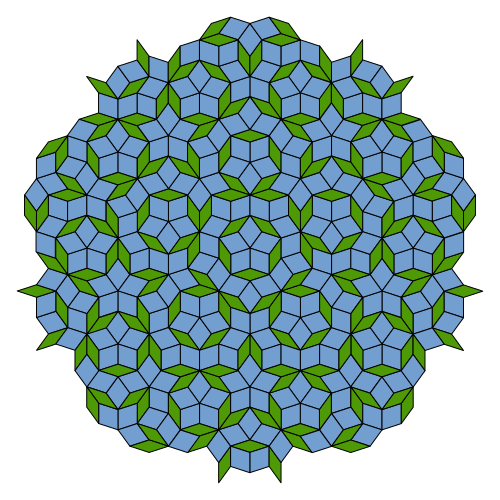
\includegraphics[scale=0.75]{./imgs/Penrose_Tiling.png}
	\caption{Замощение Пенроуза}
\end{figure}
Замещение Пенроуза не периодично, то есть \textit{апериодично}, но покрывает всю плоскость.

Основная наша цель -- доказать, что если нам дан на вход набор 11-и плиток Ванга, то
нельзя выяснить, можно ли ими замостить плоскость (то есть, эта задача неразрешима).

Задача формулируется так -- даются плиточки $ 1 \times 1 $, мы их можем помещать в целочисленные точки плоскости. Каждую из сторон мы можем помечать, например, цветами -- скажем, левую и верхнюю сторону -- красной, правую -- фиолетовой, нижнюю -- желтой. Ставить рядом можно только стороны одинакового цвета.


\begin{defn}[Замощение]
    \selectedFont{Замощение} --- это отображение $ t\colon  \mathbb{Z}^2 \to T $, где $ T $ -- набор плиток.
\end{defn}

\begin{note}
    Самих плиток бесконечно, но количество их типов -- конечно.
\end{note}

\begin{ex}
    Если плитка типа 1 -- справа и сверху синий цвет, а снизу и слева -- красный, а плитка типа 2 -- наоборот, то получится только шахматное замощение.
\end{ex}

\noindent \textbf{Вопрос, который задавал Ванг (1961):} \textit{если дан на вход набор плиток, существует ли алгоритм, проверяющий существование замощения?}

Вопрос решил его студент Berger в 1966 году, доказав неразрешимость.
Мы докажем упрощенный вариант -- замощение \textit{c зерном.}

\begin{thm}
    Задача замощения с зерном (то есть, когда выделенная плитка $ s \in T $ обязана присутствовать в замощении) алгоритмически неразрешима.
\end{thm}
\begin{proof}
    Сведем задачу остановки машины Тьюринга на пустой ленте.

    Дана $ M = (Q, \Sigma, \Gamma, , \delta, q_0, f)$, где $ f $ -- конечно. Пробел обозначаем за $B$ (blank).

    Строим $T$:
    \begin{enumerate}
        \item Плитки инициализации.
\begin{figure}[ht]
    \centering
    \incfig{init-tails}
	\caption{Плитки инициализации}
    \label{fig:init-tails}
\end{figure}
        \item  Плитки алфавита
\begin{figure}[ht]
    \centering
    \incfig{alphabet-tails}
    \caption{Плитки алфавита}
    \label{fig:alphabet-tails}
\end{figure}
        \item Плитки переходов. 
			Если есть команда $ \delta(q, a) = (p, b, t) $, то сопоставляем
			ей плитку $ (1)$.

			Если команда $ \delta(q, a) = (p, b, \rightarrow) $, то плитка  $ (2)$.
\begin{figure}[ht]
    \centering
    \incfig{delta-tails}
    \caption{Плитки перехода}
    \label{fig:delta-tails}
\end{figure}
        \item Плитки склеивания.
\begin{figure}[h!]
    \centering
    \incfig{bonding-tails}
    \caption{Плитки склеивания и пустая плитка}
    \label{fig:bonding-tails}
\end{figure}
        \item Пустая плитка, чтобы заполнить низ. 
    \end{enumerate}

    Посмотрим теперь, как плитки устроены и как мы будем делать сведение.

    Начинаем с зерна (потому что оно должно присутствовать). Что мы можем к ней приписать справа?
    Только одну из плиток инициализации (какую, видно из картинки). Слева -- аналогично.

    Какую можем вниз? Только плитку типа 5.

    Какую можем сделать при шаге машины Тьюринга? Выглядит это примерно так:
\begin{figure}[ht]
    \centering
    \incfig{step-mt}
    \label{fig:step-mt}
\end{figure}

    Все остальное -- плитки склеивания, вариантов нет.

\begin{figure}[ht]
    \centering
    \incfig{imitaion-mt}
    \caption{Имитация МТ}
    \label{fig:imitaion-mt}
\end{figure}

    Продолжается это бесконечно, потому что если машина остановится, то это будет конечное число
    шагов, и мы не сможем прилепить плитку (потому что переход будет не определен).

    Метки бесконечных строк составляют конфигурацию машины Тьюринга. Замощения существуют тогда и только тогда, когда машина Тьюринга не останавливается. Получается, если бы мы умели решать задачу замощения, то мы бы могли сказать, остановится ли машина Тьюринга.
\end{proof}

\begin{lm}
    Если для любого $ n $ существует замощение квадрата $ n \times n $, то существует замощение всей плоскости.
\end{lm}
\begin{proof}
    Аналог леммы Кенига о том, что в бесконечном дереве существует бесконечная ветвь. Или так: любая плитка встречается бесконечно много раз. Смотрим ее возмозные продолжения до квадратика $ 2 \times 2 $. Какой-то из этих вариантов встречается бесконечно много раз -- выберем его. Смотрим ее продолжения до квадратика $ 3 \times 3 $, и т.д.
\end{proof}

\begin{cor}
    Неразрешимость в купе с леммой дает существование апериодических замощений, то есть наборов плиток, для которых существуют только непериодические замощения.
\end{cor}
\begin{proof}
    Иначе можем красить увеличивающиеся квадраты $ n \times n $, либо придем к противоречию,
    либо увидим период.
\end{proof}

\begin{lm}
    Если для данного набора плиток существует замощение, периодическое в одном направлении, то существует и замощение, периодическое в двух направлениях.
\end{lm}
\begin{proof}
    Пусть $(a, b)$ -- вектор периодичности (то есть, если сдвигаем плитку на вектор $ (a, b) $ то там та же плитка).

    Рассмотрим кусочки такого размера *картинка*

    Квадратов бесконечно, способов замостить конечно, поэтому какой-то встретится два раза. При этом цвета снизу такие же,
    как и сверху (потому что период).
    Значит красным квадратом мы можем замостить все.
\end{proof}

\begin{figure}[ht]
    \centering
    \incfig{kari-tiles}
    \caption{Плитки Кари}
    \label{fig:kari-tiles}
\end{figure}
\begin{thm}[про 14 плиток]
    Плитками с картинки можно замостить плоскость, но только апериодическим способом\footnote{Подчеркнутые и не подчеркнутые цифры -- разные.}.
\end{thm}
\begin{proof}
    Надо доказать, что замощение существует, и что не существует периодического.
    *тут было очень много слов и я не успевал, нужно написать эту теорему с видео*
\end{proof}


 
\end{document}
